\documentclass{article}
\usepackage{tmlr}
\usepackage{graphicx}
\usepackage{booktabs}
\usepackage{amsmath,amssymb}
\usepackage[colorlinks=true,linkcolor=blue,citecolor=blue,urlcolor=blue]{hyperref}

% 预注册判据表的结局标记（tab_criteria.tex 使用）
\newcommand{\cpass}{\textbf{\checkmark} pass}
\newcommand{\cfail}{\textbf{$\times$} fail}
\newcommand{\cpart}{$\sim$ partial}
\newcommand{\crep}{report}
\newcommand{\cns}{\textit{not stored}}

\title{The Interference Floor: Why a Learned Corrector Degrades\\ the Prior It Was Meant to Repair}

\author{Zetao Zhang\\ Quanzhou University of Information Engineering\\ \texttt{akenman1124@outlook.com}}

\begin{document}
\maketitle

\begin{abstract}
A learned residual corrector added to an analytic prior inherits whatever the prior
already gets right and is asked to repair the rest. In the contact-rich world we study,
that division of labour fails in a way easy to miss and easy to measure: on the
free-flight windows where the prior is already exact, the head emits $0.017$--$0.027$
(normalised RMS) at every one of four prior tiers whose targets span five orders of
magnitude---closer to a constant than to anything the prior asks of it. We call this
the \emph{interference floor}. It is not universal to the architecture: an own-split
ten-seed extension on a contact-free world gives descriptive head/target means of
$0.968$, $0.953$, $0.792$ and $0.126$ across the four tiers (Table~\ref{tab:ladder_extension}),
a cross-world pattern consistent with a regime-imbalance hypothesis but not a causal
demonstration. Four training-side interventions and a decode-time gate then trace a
single false-silence-versus-damage trade-off; the gate restores parity with the
analytic prior on the thirty free-flight validation windows it scores, at a
$4.2$--$4.7\%$ window-level false-silence rate and a $12$--$21\%$ rise in
contact-regime closed-loop error. We remove three candidate explanations for the floor
and identify one term that sustains it: the closed-loop rollout loss, fit on all
windows, raises free-flight error by $1.6$--$4.7\times$ at matched fit.

Two measurements scope the result. What caps how good any of this can get is the
prior's computation class---the equations and the numerical scheme used to evaluate
them---which lowers closed-loop error from $14.26$\,px to $0.49$\,px when swapped for
the class that generated the data. And the head is not worthless in general: when the
prior's parameter is wrong or a force is unmodelled, it removes $89$--$97\%$ of the
error. Where the prior is already exact the correction is unneeded, and the floor is
the cost of asking for it---measured here, not explained. The identification result
that accompanies the computation-class claim is a stable local optimum under one
optimizer protocol, not a global one. Preregistered criteria, guard-bound numbers and a
measured reproduction floor accompany all of it, including the criteria our claims
failed.
\end{abstract}

\section{Introduction}

A world model that is meant to support control has to survive closed-loop rollout: the model consumes its own predictions, step after step, and errors compound. The standard workflow trains on one-step prediction, reports a one-step metric, and hopes. The question this paper asks is narrower than ``are world models useful''. It is: given a fixed architecture family and a fixed data budget, what decides whether a learned model survives the step from one-step fitting to closed-loop rollout?

Three answers circulate in practice. The first is architectural: give the model structure---gating, phase variables, symbolic priors---and it will roll out better. The second is the training recipe: add a rollout loss, tune the schedule. The third is rarely treated as a measured variable at all: the fidelity of an analytic prior's \emph{computation class}, by which we mean the pair of equations and the numerical scheme (integrator, step size, sampling) used to evaluate them. A prior can be exact as mathematics and still be wrong as code, if its discrete map differs from the map that produced the data. A reader may object that, in simulation, matching the generating integrator is trivially the right thing to do. It is the right thing, and it is not trivial to know what to match. Our own preregistered analytic basis for the ball engine was wrong---we had assumed the semi-implicit form the scheme's name suggests, while the engine integrates positions before velocities---and that discrepancy is larger than every ladder gap we resolve except the coarsest (\S\ref{sec:platform}).

Measuring this properly takes an instrument, so we built one. Two simulated worlds---an underactuated double pendulum and a bouncing-ball arena---with a shared architecture family in which the residual head, the trunk, and the data budget are held fixed while the prior is swapped through a registry of four integrator tiers. Twelve preregistrations, written before the runs, fix the criteria. Every number in this paper is reproduced by a script from a stored JSON and checked by guard tests, and every claim above the reproduction floor is scoped by a measured retraining variance whose worst case ($15\%$ on the five-step pendulum metric) is reported in \S\ref{sec:limitations}.

The findings are ordered by how they bear on that question, and the first one is the
problem rather than the answer. On the windows where the exact prior is already
perfect, the residual head is supposed to output zero; the supervision there is zero to
four decimals, and the head's output is not. It emits $0.017$--$0.027$ (normalised RMS)
at every one of four prior tiers whose targets span five orders of magnitude---at the
exact tier, $1.4\times10^{5}$ times its own target. The head is closer to a constant
than to anything the prior asks of it, and this noise erases the analytic ladder in the
trained arms and compounds under feedback. We call it the \emph{interference floor},
and it is not a property of the architecture: the same model trained on a contact-free
world has no comparable floor: its own-split ten-seed sensitivity extension gives
head/target means of $0.968$, $0.953$, $0.792$ and $0.126$ across the four tiers. It reuses
the original seeds and is not an independent replication (Table~\ref{tab:ladder_extension}).
This pattern is consistent with a regime-imbalance hypothesis, not a causal identification.
The title's ``why'' refers to the terms the interventions below identify---the training
mixture that sets the floor and the closed-loop rollout loss that sustains it
(\S\ref{sec:silence})---not to the cross-world boundary, which remains a labelled hypothesis.
We tried five interventions across four preregistrations---loss reweighting, an
end-to-end gate, a supervised gate, a loss-mass dose curve, and decode-time hard
gating---and each moved the error somewhere else: together with the decode rule they
trace one curve, a trade between silencing the head on free-flight windows and damaging
contact windows, whose exchange rate we quote. The decode rule is the useful end of
that curve, restoring closed-loop parity with the analytic prior on the thirty
free-flight validation windows it scores.

Two measurements frame that result. What caps how good any of this can get is the prior
ladder: in the pendulum world, exchanging the coarse integrator of the prior for the one
that generated the data moves the trained arm's one-step error from 0.969\,px to
0.037\,px and closed-loop error from 14.26\,px to 0.49\,px (Table~\ref{tab:ladder}).
The original three-seed means differ by factors of 26 and 29. In the ten-seed extension,
the one-step ratio is smaller (17.7$\times$) because the coarse-tier estimate is seed-sensitive
(Table~\ref{tab:ladder_extension}); the architecture is held fixed throughout. The same experiment in the ball world reproduces analytic
predictions to four decimal places, and the exact prior there is not merely close to the
engine: over five closed-loop steps it \emph{is} the engine, to
$3{\times}10^{-5}$\,px per step on the filtered free-flight slice. In the pendulum world a learned model with 401k parameters matches this floor
and cannot improve on it; in the ball world it does not, and that asymmetry is the subject of \S\ref{sec:silence}. The recipe, meanwhile, multiplies within the floor: a rollout
loss repairs a collapsing arm by $41\times$ but changes the exact-prior arm by nothing,
and there is a dose above which more single-step loss reverses closed-loop performance
outright. Symbolic structure costs accuracy in every form we tried---gated experts
across three gating generations, and label supervision in a two-by-two that
separates it from capacity (0.269\,px, 6/6 seeds)---yet when
the floor is exact, that harm is absorbed almost perfectly (ratio $0.0005$). And the
head is not worthless in general: when the prior's parameter is wrong or a force is
unmodelled, the same head removes $89$--$97\%$ of the error. The floor is the price of
correction on the one regime where no correction is needed.

This paper is a study of two simulated worlds, not a benchmark. The scale is deliberately small and the claims are scoped accordingly. What the small scale buys is control: every factor that could move the numbers is either fixed, preregistered, or guarded by a test. Our contributions:
\begin{itemize}
  \item \textbf{C1 --- The interference floor.} In the contact-rich world the residual head's output on the windows where the prior is already exact is set by the training mixture, not by the prior: $0.017$--$0.027$ across four tiers whose targets span $10^{5}$, and $1.3$--$1.4\times10^{5}$ times its own target at the exact tier. The same architecture in a contact-free world shows descriptive own-split head/target means of $0.126$--$0.968$ in a ten-seed sensitivity extension that reuses the original seeds; this is not an independent replication, and it is consistent with, but does not identify, a role for regime imbalance (\S\ref{sec:silence}; terms and units in Appendix~\ref{app:notation}).
  \item \textbf{C2 --- The exchange rate, and one term that sustains it.} Four training-side interventions and a decode rule lie on one false-silence-versus-damage curve, which we quote as a measured rate; three candidate explanations are removed and the closed-loop rollout loss is identified as a term that actively counteracts silence (\S\ref{sec:silence}).
  \item \textbf{C3 --- The floor the prior sets.} The prior's computation class caps what any residual head can reach: swapping it for the class that generated the data lowers closed-loop error from $14.26$ to $0.49$\,px, and in the pendulum a zero-parameter prior with the engine's integrator ties a 401k-parameter learned model. The ball world does not reproduce that tie (\S\ref{sec:floor}, \S\ref{sec:silence}).
  \item \textbf{C4 --- Correction is worth what the prior is wrong learnably.} On a control where the prior is merely discretised the head returns $-0.4\%$; when the prior's parameter is wrong or a force is unmodelled the same head removes $89$--$97\%$ of the error, and freezing the trunk does better still (\S\ref{sec:when}).
  \item \textbf{C5 --- Symbolic structure is a measured tax.} Within this architecture family, symbolic structure---in gating and in supervision---consistently costs accuracy, and the cost vanishes once the floor is exact (\S\ref{sec:substitute}).
  \item \textbf{C6 --- Methodology as a working instrument.} Preregistered criteria, single-source numbers bound by guard tests, and a measured reproduction floor caught three of our own wrong conclusions before publication, and a single retrained arm prices the floor per metric (\S\ref{sec:platform}, \S\ref{sec:limitations}, \S\ref{sec:repro}).
\end{itemize}

\section{Related Work}

\paragraph{Reuse-and-correct methods.} A family of systems couples an analytic simulator with a learned corrector: alternating neural integrators for legacy simulators \citep{ani2026}, differentiable-simulator augmentation \citep{neuralsim2021}, residual physics for throwing \citep{tossingbot2019}, material-aware residual world models for deformable objects \citep{physcore2026}, and end-to-end identification of rigid-body dynamics from vision \citep{pinwm2025}. These works answer \emph{how to repair}. We ask the adjacent question that their evaluations presuppose: \emph{what determines whether the repair is possible, and what the repair costs}. Our interference result is a caveat their architectures inherit---the corrector's noise on the prior's home regime---and our decode-time rule is one measurable answer.

\paragraph{Structure-preserving learning.} Hamiltonian and Lagrangian networks build the integrator into the learner \citep{hgn2019,chnn2020,se3hode2021}. The concern for long-horizon stability is the same as ours; the causal question is different. We do not ask whether a learned model can be made to respect structure, but how much of closed-loop error is explained by the prior's computation class once structure is present as a candidate explanation and rejected.

\paragraph{Rollout error accumulation.} That autoregressive error compounds is a known and much-analysed property of learned dynamics \citep{pderefiner,mbpo2019,swazinna2021}. We contribute the controlled version: with the architecture and data fixed, the compounding term is governed by the prior's fidelity, it saturates at the floor, and the training-side levers that reduce one component of it reliably inflate another (\S\ref{sec:silence}).

\paragraph{Auxiliary-task interference.} Capacity loss from auxiliary losses \citep{lyle2021}, gradient-magnitude balancing across tasks \citep{metabalance2022}, and expert-utilisation pathology in mixture-of-experts \citep{deepseekv3,auxlossfree2024} are the nearest neighbours of our interference floor. The instance here is new---a residual head that will not stay silent where an exact prior leaves it nothing to do---and we test the obvious fixes causally rather than proposing another balancer.

\paragraph{Handing authority back to a deterministic floor.} Handing authority to a fallback controller is established in control: predictive safety filters verify a backup trajectory online and revert to it when a learned policy risks constraint violation \citep{wabersich2021}, and control-barrier-function filters modulate a nominal controller to keep a safe set invariant \citep{ames2019}; abstention and conformal wrappers extend the idea under uncertainty. Our decode-time gate is that idea applied to a dynamics world model, with two additions: the regime indicator is physically interpretable (a contact indicator, not an epistemic score), and the cost of handback on in-distribution performance is measured as an explicit exchange rate rather than left implicit.

\paragraph{Discretisation bias is classical; its size beside architecture is not.} That a model estimated from sampled data of a continuous-time process absorbs the discretisation into its parameters is classical in system identification \citep{ljung1999}. Our identification experiment reproduces exactly that behaviour ($\hat g = 705.7$ against a generating $900$ on the clean world, and $871$--$886$ against $1125$ on the perturbed ones), and we read the classical result as the reason to expect it rather than as a finding. What the classical treatment does not supply is the comparison this paper is built around: with architecture, data, recipe and seeds fixed, how large the absorbed bias is next to the levers a practitioner actually chooses between---the prior's computation class, symbolic structure, and loss geometry---and how it translates into closed-loop error.

\paragraph{Implicit identification is also classical; its price on the easy regime is not.} A residual head that learns a state-dependent correction to a parametric prior is doing online parameter estimation implicitly, and that too has a classical lineage \citep{ljung1999}: recursive least squares and Kalman-filter estimators update a parametric model as data arrive. The correspondence is behavioural rather than structural---our head carries no parameter state or covariance---and \S\ref{sec:when} shows it directly: when the prior's parameter is wrong by $25\%$, a head---trained on a trunk that never saw the mismatch---recovers $93\%$ of the closed-loop error, which is what an implicit estimator should do. The classical literature tells us to expect the recovery; what it does not price is what the same estimator does on the windows where the parameter is already right. That price is the subject of \S\ref{sec:silence}, and it is the part of this paper we take to be new.

This paper studies \emph{dynamics-level} world models for control; video- and LLM-scale world models evaluate on different semantics \citep{wm_survey2026} and are out of scope.

\section{Experimental Platform}\label{sec:platform}

\subsection{Two worlds}

\textbf{Pendulum.} An underactuated double pendulum in the acrobot configuration: two links ($L=80$\,px, point masses 2.0 and 1.0), gravity 900\,px/s$^2$, one normalised elbow torque bounded at 28{,}000. Ground truth integrates the Lagrangian equations with RK4 at 0.01\,s and samples at 20\,Hz. The state is 25 dimensions per window step: two 11-dim object segments (position, angle as sin/cos, linear and angular velocity, constant attributes) plus a three-channel contact block. Three thousand episodes of 10\,s. The prior is torque-driven and contact-free by construction, which makes this world the clean instrument: its exact tier can be checked against the engine frame by frame.

\textbf{Ball.} A planar arena simulated with a rigid-body engine: three dynamic bodies, static obstacles in eight visible slots, gravity 900\,px/s$^2$, actions recorded as per-body net impulses over each 0.05\,s interval, applied as constant forces at every 0.01\,s engine step. Fifty thousand episodes of 200 frames. The state assembles to 116 dimensions (33 object, 80 obstacle, 3 contact). This world adds what the pendulum lacks: contact. Its free-flight segments are the only place where a contact-free prior can be exact, and its engine turned out to be instructive in its own right, for a reason we did not expect. The arena runs on pymunk/Chipmunk2D, whose documentation states that it ``uses standard Euler to perform the integration'' and spells out the order the integrator works in: positions are integrated \emph{before} velocities \citep{pymunk2025}. A transfer therefore accumulates $10a\Delta t^2$ rather than the $15a\Delta t^2$ that integrating velocities first (semi-implicit, and the form the scheme's name suggests) would give. Our preregistration had assumed the semi-implicit form; the data forced the correction, and at 900\,px/s$^2$ the two signatures differ by 0.45\,px per transfer along gravity ($0.32$\,px pooled over the six position dimensions)---twice the finest gap the ball ladder resolves in \S\ref{sec:floor} (0.159\,px, pooled). The lesson is not that this engine's documentation and code disagree. It is that a plausible prior about an engine's discrete map can be wrong by more than the effect being measured, and that only the data settle it. All quantities are in the engine's native pixel units; converting them would add a constant to every tier and cannot change a comparison, so we do not.

\subsection{Architecture family}

All arms share a GRU trunk (hidden 256 unless stated) with LayerNorm, consuming the assembled window ($L{=}8$ past frames). The residual parameterisation is fixed throughout: the head predicts a correction to the prior's output, $\mathrm{pred} = \mathrm{prior}(s_t, a_t) + \mathrm{head}(h_t, a_t)$, with the head's final layer small-initialised so that training starts at the prior. Around this trunk we register fifteen arms for the pendulum (pure learning, strong MLP, JEPA-style, gated, ablations, four analytic tiers) and the trained ladder plus two silence mechanisms for the ball. Parameter budgets are levelled to within $\pm 10\%$ of the base arm; the wiring of every arm is asserted from its state dictionary, not from its configuration, by guard tests (\S\ref{sec:repro}). Across the arms reported here, model sizes run from 339k to 615k parameters: the pendulum models sit at 387k--431k, the ball models at 598k with the two gate arms of \S\ref{sec:silence} at 615k, and the capacity ablations of \S\ref{sec:substitute} span 339k--470k by design rather than by budget.

\paragraph{Training recipe.} Unless stated, every arm is trained with AdamW (weight decay $10^{-5}$) and a cosine-decayed learning rate, using model selection on the validation split. The pendulum arms use learning rate $10^{-3}$ and batch $256$; the ball arms use learning rate $3\times10^{-4}$ and batch $1024$. Both use $60$ epochs and cap the training set at $150$k windows per epoch for cost. The closed-loop rollout horizon is $K{=}5$ for the pendulum and $K{=}3$ for the ball ($L{=}8$ past frames throughout); identification experiments use Nelder--Mead rather than this recipe. The per-arm settings are recorded in the released configuration files.

\subsection{The prior registry}

Each world has a registry with four prior tiers---for the pendulum, semi-implicit Euler at 0.05\,s, Euler at 0.01$\times$5, RK4 at 0.05\,s, RK4 at 0.01$\times$5; for the ball, the legacy closed-form parabola, explicit Euler at $0.05{\times}1$, RK4 at $0.05{\times}1$, explicit Euler at $0.01{\times}5$. The registry is the single implementation: a numpy path builds training targets, a torch path serves evaluation, and a test asserts the two agree to within $10^{-4}$ and that the default tier reproduces the historical implementation bit for bit. The tier used to build the residual target during training is the same tier the model evaluates with; a mismatch there would silently invalidate every comparison, so it is guarded, not promised.

\subsection{Protocol}

Every experiment in this paper that belongs to one of the twelve preregistered slots ran under a preregistration written before the first run: design, seeds, thresholds with their calibration source, stopping rules, and what counts as a crashed run. Comparisons are paired by seed; crashed runs stay in the analysis (ITT) and their rate is reported. In practice no run crashed: every slot that stores the field records an ITT rate of $0.0$ (S0b, S1b, S1d, S1e, S1f), and the supervision $2\times2$ records $0/24$. There is one exception to that accounting, and it applies to the gating series of \S\ref{sec:substitute}, which predates the twelve preregistrations: those arms additionally report stable-run means with collapsed runs excluded, because a collapsed run's saved checkpoint is systematically worse than a completed one's. The report that defines them (\texttt{E1a\_corrected\_report.json}) also carries the full-sample reading and marks the criterion \textsc{disagree} rather than choosing between the two; the crash rates that rule produces are unequal across arms ($0/10$, $1/10$, $3/10$ for three of the variants), which is why both readings are reported rather than one. The run-to-run reproduction floor was measured by retraining configurations from identical settings and comparing to the first runs. On one-step error it is small---$0.5\%$ on the retrained arm, and the analytic prior reproduces bit for bit---and on the pendulum's closed-loop $k{=}2$ it is $0.2\%$. On the five-step closed-loop metric of \S\ref{sec:floor} it is not: the same arm, seed and hardware retrained to a different selected epoch moves from $14.07$ to $16.18$\,px, $15\%$. We therefore treat the $29\times$ ladder separation of Table~\ref{tab:ladder} as the only closed-loop gap we resolve on that five-step metric, and quote smaller closed-loop effects only on metrics whose own reproduction floor we measured; \S\ref{sec:limitations} carries the per-quantity numbers. Our three-to-six seed budget is at the low end of what the power-analysis literature recommends \citep{colas2018}, which is why the guard is directional replication against preregistered absolute thresholds rather than significance claims. Every headline number in this paper descends from a stored JSON report through a single build script; 43 guard tests (prior-registry cross-checks, document-to-JSON consistency, checkpoint-naming and overwrite protection, wiring assertions read back from state dictionaries) make divergence between the paper's numbers and the artifacts a test failure rather than a possibility. Twelve preregistrations accompany the paper, the mechanism probe of \S\ref{sec:silence} included. Three of our own earlier conclusions were overturned inside this protocol before publication---a gating advantage, a loss-quality claim, and a dose--response expectation---and all three are described in the body (\S\ref{sec:substitute}, \S\ref{sec:silence}, \S\ref{sec:discussion}) because they are part of the result.

\section{The Prior Ladder Sets the Floor}\label{sec:floor}

\subsection{A ladder in the pendulum world}

We first trained the residual architecture on the pendulum world with four priors, everything else fixed (60 epochs, three seeds). One-step error follows the prior tier monotonically: 0.969, 0.196, 0.136, 0.037\,px as the integrator moves from coarse Euler to the engine's own RK4 scheme; closed-loop error at five steps follows it from 14.26 to 0.49\,px (Table~\ref{tab:ladder}). One caveat belongs on that second column: the coarse-prior arm's five-step value carries $15\%$ run-to-run variance under retraining (\S\ref{sec:platform}), so the ladder is quoted as a $29\times$ separation and not as four precise numbers; the exact tier's own cross-seed standard deviation is $0.009$\,px, well below the smallest difference the ladder rests on ($0.06$\,px). The exact tier beats the preregistered thresholds on all four criteria (Table~\ref{tab:criteria}). Two details deserve emphasis. The residual head's contribution to closed-loop error is not stable---across tiers it ranges from a 10\% improvement over its own prior to a 50\% degradation---while the prior tiers themselves differ by $32\times$ (the trained arms, $29\times$). And the exact tier is much less variable than the coarse and intermediate tiers: in the original three-seed table, its closed-loop SD is 0.009\,px versus 1.3--2.4\,px in the middle tiers. The ten-seed extension retains that contrast (0.008\,px at the exact tier against 0.8--3.2\,px in the middle tiers) while also showing substantial split-plus-optimization variation in the coarse and intermediate arms (Table~\ref{tab:ladder_extension}; \S\ref{sec:limitations}).

\begin{table}[t]
\centering
\caption{The pendulum prior ladder (three seeds, mean). Everything except the prior tier is held fixed; the pendulum's Euler tiers are semi-implicit, where the ball's are explicit (\S\ref{sec:platform}).}
\label{tab:ladder}
\small
\begin{tabular}{llcccc}
\toprule
Arm & Prior tier & one-step (px) & closed-loop $k{=}5$ (px) & prior one-step & prior $k{=}5$ \\
\midrule
trained & Euler@.05$\times$1  & 0.969 & 14.26 & 3.373 & 15.80 \\
trained & Euler@.01$\times$5  & 0.196 & 4.87  & 0.522 & 3.24 \\
trained & RK4@.05$\times$1    & 0.136 & 2.19  & 0.147 & 1.68 \\
trained & RK4@.01$\times$5    & \textbf{0.037} & \textbf{0.49} & 0.038 & 0.49 \\
\midrule
0-param & RK4@.01$\times$5 (exact) & 0.038 & 0.49 & --- & --- \\
\bottomrule
\end{tabular}
\end{table}

The original three-seed result is retained above as Table~\ref{tab:ladder}; Table~\ref{tab:ladder_extension} places it beside the ten-seed sensitivity extension. The extension reuses seeds 42--44 and adds 45--51, so it is not an independent replication. Under the expanded sample the one-step means are 0.665, 0.172, 0.097 and 0.038\,px; the coarse estimate moves appreciably. We use Table~\ref{tab:ladder} for the preregistered result and the extension table for descriptive sensitivity.

% AUTO-GENERATED by paper/tables/build_ladder_extension_table.py
\begin{table}[t]
\centering
\caption{Original three-seed pendulum ladder and its ten-seed extension. The ten-seed set reuses seeds 42--44 and adds 45--51; it is a within-dataset sensitivity extension, not an independent replication. Table entries are means in px; the extended column gives mean $\pm$ descriptive SD using each checkpoint's own validation split, so it combines optimization and split variation. The final column is the descriptive mean ratio of head RMS to target RMS across the ten own-split runs; these runs share source episodes and are not independent replicates. The former common-split analysis is retained only as an audit artifact.}
\label{tab:ladder_extension}
\small
\begin{tabular}{lrrrrr}
\toprule
Prior tier & $n{=}3$ one-step & $n{=}10$ one-step & $n{=}3$ $k{=}5$ & $n{=}10$ $k{=}5$ & head/target \\
\midrule
Euler@.05$\times$1 & 0.969 & 0.665 $\pm$ 0.339 & 14.26 & 15.40 $\pm$ 2.53 & 0.968 $\pm$ 0.043 \\
Euler@.01$\times$5 & 0.196 & 0.172 $\pm$ 0.035 & 4.87 & 4.98 $\pm$ 3.18 & 0.953 $\pm$ 0.024 \\
RK4@.05$\times$1 & 0.136 & 0.097 $\pm$ 0.043 & 2.19 & 1.68 $\pm$ 0.77 & 0.792 $\pm$ 0.070 \\
RK4@.01$\times$5 & 0.037 & 0.038 $\pm$ 0.001 & 0.49 & 0.50 $\pm$ 0.01 & 0.126 $\pm$ 0.008 \\
\bottomrule
\end{tabular}
\end{table}


\subsection{The zero-parameter ladder crosses engines}

The trained ladder conflates two things: the quality of the prior and whatever the head does with it. So we removed the head. Four zero-parameter priors were evaluated on the ball world's contact-free transfers, with the pendulum's three-tier analytic validation as precedent. The scored subset is the 6{,}597 transfers that pass a contact-flag and velocity-consistency filter, out of 64{,}463 free-flight transfers in the slice---the filter keeps about one transfer in ten, so it is load-bearing and we report both slices below.

The engine check comes first and it is the reason to trust everything after it. The ball engine's exact tier---explicit Euler at 0.01\,s, five substeps, constant per-step forces---reproduces the recorded transitions to $3{\times}10^{-5}$\,px one-step, and rollouts over five closed-loop steps reach $1.4{\times}10^{-4}$\,px. A zero-parameter prior reproduces the learned data-generating process to float32 precision ($3\times10^{-5}$\,px per step) at deployment sampling (Fig.~\ref{fig:ladder}b).

The ladder itself, on free-flight windows: the legacy closed-form parabola and the RK4 tier tie at 0.1591\,px; the same-family coarse tier sits at 0.6364\,px. Both values were predicted analytically before the run: the parabola and RK4 are the exact solution of the constant-acceleration problem and miss the engine's per-transfer position gain by $2.5a\Delta t^2$ along the gravity axis (0.225\,px at $a{=}900$), the coarse tier by $10a\Delta t^2$ (0.9\,px); pooled over the six position dimensions, of which gravity moves three, the predicted pos-RMSE is these over $\sqrt{2}$---0.1591 and 0.6364\,px---and the measurements reproduce them to the fourth decimal. Two readings matter. First, the mathematically exact solution is not the computationally matched one: the parabola solves the ODE perfectly and is still 0.159\,px wrong at every step, because the engine's discrete map is not the flow. Second, matching the family without matching the step size does not help; the same-family tier is the worst of the four. The filter that defines these numbers decides the headline, so both slices are reported. On the filtered slice the exact tier's one-step error is $3{\times}10^{-5}$\,px against the coarse tier's 0.6364\,px, a factor of $2{\times}10^{4}$. On the unfiltered slice---all 64{,}463 free-flight transfers---the same tier's one-step error is 0.4355\,px against the coarse tier's 0.4647\,px, only $6\%$ better. The engine-matched prior is exact on the transfers that survive the velocity-consistency filter and near the coarse tier on those that do not, so we claim float32-exactness only for the filtered slice; only the filtered slice carries closed-loop numbers (1{,}398 closed-loop windows). On mixed windows that include contact, the four tiers land in 0.90--1.21\,px and the analytic ordering does not survive: the engine-matched tier (1.107\,px) is $22\%$ worse than the coarse tier (0.905\,px). Contact mismatch asserts itself there as a second, additive error source that no integrator choice addresses.

\begin{figure}[t]
\centering
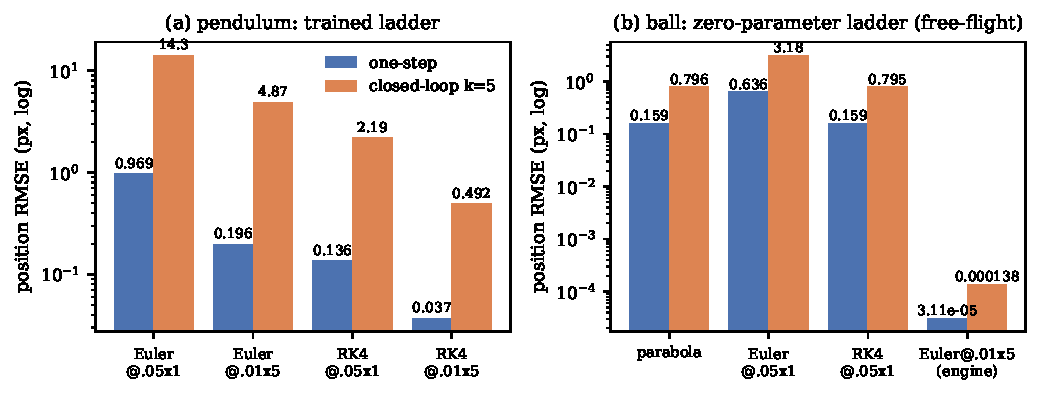
\includegraphics[width=\textwidth]{figs/fig1_floor_ladder.pdf}
\caption{The prior ladder in both worlds, log scale. (a) Pendulum: trained residual arms, four prior tiers (Table~\ref{tab:ladder}). (b) Ball: zero-parameter analytic priors on contact-free windows, with the engine-exact tier at $3{\times}10^{-5}$\,px. Analytic predictions (\S\ref{sec:floor}) match the measurements to the fourth decimal.}
\label{fig:ladder}
\end{figure}

\subsection{A parameter-compensation basin under one optimizer protocol}\label{sec:basin}

The identification experiments (their architecture is also used in \S\ref{sec:silence}) illustrate a possible consequence of computation-class mismatch, but do not establish a general identification law. Under the registered Nelder--Mead setup, the clean-world fit returns $\hat g=705.7$ when the generating value is $900$. To test whether this value depends on the single starting point $g{=}1200$, we re-ran the identical data, windows, objective and optimizer from nine starting values $g_0\in\{600,\dots,1400\}$ (step 100). All nine runs converge; their end points lie in $[705.4,\,705.9]$ (median $705.8$, a spread of $0.07\%$), and their objective values agree to the sixth significant figure, so the bias does not come from the choice of start. This is a local-minimum statistic within that band, not a certificate of global optimality: the grid stops at $1400$ rather than the bound of $1500$, and the search gives no proof that no lower objective exists elsewhere. The same optimizer returns $870.9$, $880.7$ and $886.4$ on three independently regenerated worlds at $g{=}1125$, and $957.3$, $961.4$ and $958.5$ under the refined computation class; those runs were not repeated across starting values and are a post-hoc sensitivity analysis of the stored protocol. We therefore describe the clean-world value as a stable optimizer output consistent with a parameter-compensation basin under this protocol, not as a sample-independent law, and make no multi-start claim for the regenerated worlds. Discrete-time estimates can absorb discretisation error, a classical observation \citep{ljung1999}.

\subsection{What the floor buys}

With the exact prior in place, the residual head has nothing measurable to learn in the pendulum world: the three-seed trained mean reaches 0.037\,px against its prior's 0.038, and the closed-loop means are 0.49 against 0.49. The ten-seed extension gives 0.038\,px (sd 0.0006) one-step and 0.497\,px (sd 0.008) at $k{=}5$ (Table~\ref{tab:ladder_extension}). A 401k-parameter learned model is numerically close to the zero-parameter prior at this tier; we do not interpret the ten-seed extension as a new preregistered equivalence test. This tier is exact with respect to the engine's integrator, not to machine precision, and the residual gap is a property of the labels. The generator updates the elbow torque every 0.01\,s inside a 0.1\,s ramp, while each action label records only the last value of its 0.05\,s interval, so the $18.8\%$ of windows that sit inside a transition carry an intra-interval torque schedule no prior can observe. Measured with the same exact integrator, the one-step error is 0.018\,px on transition-free windows and 0.079\,px on the remainder; the 0.06\,px difference between them accounts for the contribution of the unobservable schedule, and it is why this tier levels off at 0.038\,px instead of continuing toward zero. A full-observability control confirms the attribution: regenerating the same 3{,}000-episode protocol with the torque held constant within each 0.05\,s sample interval---so the action label determines the applied torque---collapses the exact-tier prior's one-step floor from 0.038 to $3.0\times10^{-6}$\,px, and the same-recipe arm retrained on the control data reaches $2.5\times10^{-4}$\,px: over $150\times$ below the original plateau, though still above the control prior's own machine-level floor. The plateau is the information limit of the label schedule, not a property of the trained model. The ball world has no such component because its action schedule is fully observable, and that is where the engine-matched prior reaches float32 exactness (\S\ref{sec:floor}). This is the clean statement of C3: on this contact-free world and at this computation class, the residual head adds no measurable improvement. The rest of the paper is about what happens when the prior is not exact.

\section{The Interference Floor and the Cost of Silence}\label{sec:silence}

\subsection{The interference floor}

The ball world's trained ladder should, if \S\ref{sec:floor} holds for trained arms, order itself like the analytic ladder. It does not. Four trained arms---same architecture, same data, priors differing by the analytic ladder of \S\ref{sec:floor}---land at $0.86 \pm 0.05$, $0.87 \pm 0.05$, $0.98 \pm 0.22$ and $0.86 \pm 0.04$\,px on free-flight windows (three seeds each), unordered and, against their seed spread, indistinguishable, when their priors sit at 0.16, 0.64, 0.16 and $3{\times}10^{-5}$. The trained arm of the exact prior is roughly $3{\times}10^{4}$ times worse than its own prior on the windows where that prior is perfect (Fig.~\ref{fig:interference}a).

The probe in Table~\ref{tab:probe} locates the error. On free-flight windows the residual target for the exact-prior arm is 0.0000 (normalised RMS, four decimals); the head outputs 0.0197. The coarse-prior arm's target on the same windows is 0.0036---the analytic 0.159\,px, as \S\ref{sec:floor} predicts---and its head outputs 0.0203. Across all four prior tiers and three seeds the head emits $0.017$--$0.027$ on these windows, a $1.6\times$ range, while the corresponding tier means span only $1.2\times$, and the priors themselves span five orders of magnitude and the targets the head is asked to reproduce span $10^{5}$: on the exact tier it emits $0.0197$ where its target is $1.4\times10^{-7}$, a ratio of $1.4\times10^{5}$. The head is closer to a constant than to anything the prior asks of it. We call this quantity the \emph{interference floor}: a noise term in the trained arm's error that is not read off the prior, and that we hypothesise is set by the training mixture. In the ball world, contact windows carry the loss, and silence is not learned. On the pendulum, an own-split ten-seed sensitivity extension finds descriptive head/target ratios from $0.126$ to $0.968$ across the four tiers (Table~\ref{tab:ladder_extension}); it reuses source trajectories and original seeds and is not an independent replication. This contrast is consistent with a regime-imbalance hypothesis, but neither identifies a universal boundary or establishes its causal mechanism. A mechanism ablation points at the source: excluding free-flight windows from the gradient entirely ($w_{\text{ff}}{=}0$) leaves the noise at $0.0213$ (normalised RMS, seed 42) against the three-seed S1c baseline mean of $0.0186$---a shift of $+14\%$ against that mean, or $+8\%$ against the same-seed baseline reading of $0.0197$ (Table~\ref{tab:probe})---while upweighting them ($\times10$) halves it, to $0.0089$ at seed 42 against the three-seed mean of $0.0095$. The $w_{\text{ff}}{=}0$ arm is a single run on a single seed, so the two comparisons mix $n{=}1$ with $n{=}3$; both are given above rather than one, and we read the result as a mechanism probe rather than a measurement, since the shift sits above the one-step reproduction difference ($0.5\%$) but well below the five-step reproduction floor ($15\%$). Its evaluation is stored as \texttt{S1g\_report.json}, produced by \texttt{eval\_s1g.py} from the preregistered checkpoint on the S1c protocol. By \emph{silence} we mean the head's quiescence on the regime where the prior is already exact---output near zero where the target is near zero---and the rest of this section is an attempt to purchase it. Both preregistered criteria of this slot failed as written---the trained ladder does not inherit the analytic order (S1b-1) and the head does not reach the $0.50$\,px closed-loop silence bound (S1b-3, $2.04$\,px)---and those two failures are the finding of this section, not a deviation from it.

\subsection{Why the head ignores the prior: what is ruled out}
\label{sec:flooranalysis}

A constant-output head is a strong claim, so we tried to derive the constant and
failed twice. Two candidate accounts of the $0.017$--$0.027$ band were tested on
the same window set and both are rejected. First, representation cost: if the head
is fit on contact windows and extrapolated to free-flight inputs, the free-flight
output should scale as the head's local Lipschitz constant times how far free-flight
hidden states sit from the contact subspace times the contact target. Across 16
arm--seed pairs the predicted and actual values correlate at $\log$-$\log$
$r{=}{+}0.30$ with a median ratio of $0.53$. Second, loss mass: the free-flight
share of the state loss is not the driver either---the head's directional leverage
along the free-flight direction correlates with its output at $r{=}{-}0.04$ across
19 runs, and the range of outcomes is only $1.6\times$. A third intuition also fails:
the head is not flat on free-flight inputs. Its Jacobian norm on free-flight inputs is $0.66$ for the exact-prior arm against
$0.43$ on contact windows ($1.5\times$; the six-arm mean is $0.89$ against $0.43$,
with a wide $0.23$--$2.9$ spread driven by the gated arm), so the head is not flat
in the free-flight direction and merely happens to emit a small value at the specific hidden states the data supplies.
Nothing about the observed level follows from Lipschitz or overlap geometry.

What the floor does respond to is how much loss mass free flight is given, and what
stops it responding is identifiable. Freezing the trunk of the exact-prior arm and
refitting only the head under the training objective's own Huber state loss, sweeping
the free-flight window weight $w_{\text{ff}}$, gives a monotone response over
$2.4\times$: $1.41$, $0.96$, $0.91$, $0.89$, $0.75$, $0.64$ and $0.58$ of the
unmodified head's free-flight output as $w_{\text{ff}}$ runs from $0$ to $100$
(Fig.~\ref{fig:floor}). Even at $w_{\text{ff}}{=}100$---where free-flight windows
carry $83\%$ of the effective loss mass---the head still emits $0.58$ of the original
noise, and the contact-window head output drifts up by $16\%$ over the same range. That
contact cost is at the edge of the reproduction floor rather than a decisive trade, but
it is a cost and we do not read the knob as free. Silence is not
reachable on these features by weighting alone. The endpoint is not tightly
determined, and we report the spread rather than the more flattering end of it. Across
five refits of the same configuration---varying the random-number execution order and
the size of the training pool from $120$k to $400$k windows---the attainable
free-flight output lands between $0.28$ and $0.58$ of the unmodified head, and training
the trunk as well as the head does not improve on that: at the same weight it plateaus
at $0.47$ while actually improving the contact regime to $0.92$. Freezing the trunk is
therefore a probe choice rather than the source of the floor, and the honest statement
is a band of roughly $0.3$--$0.6$ for what this arm reaches with the knob alone.

One term in the objective does more work than any weight setting, and it is the term
this paper had not varied. Adding the closed-loop rollout loss to the frozen-trunk
refit---same trunk, same weights, same schedule, the only difference being
$w_{\text{roll}}{=}0.3$---raises the free-flight error by $1.6$ to $2.8\times$ at
matched global fit, and by $4.7\times$ in the run where the two cells also share an
execution path. Because the comparison is made at matched total loss, the rollout term
is not merely making the head worse: it relocates where the error sits, pulling the
head off the silence it would otherwise find. That is the mechanism the previous
paragraph was missing, and it is specific: the rollout loss is fit on all windows
rather than on the free-flight subset, so nothing in it rewards silence. The practical
reading is unchanged and is what the rest of the section builds on---silence is
purchasable, but only up to a ceiling that weighting alone does not move, and one
objective in the standard training recipe actively resists it. That is why the
decode-time rule exists.

% AUTO-GENERATED by paper/tables/build_arms_table.py
\begin{table}[t]
\centering
\caption{Every arm of \S\ref{sec:silence}, all on the exact-prior branch, three
seeds (means, px). \emph{FF} = contact-free windows; \emph{mixed} = windows
including contact; $k{=}3$ = closed-loop rollout on FF windows. Rows are grouped
by intervention family: five families, seven trained arms. The decode rule acts
at rollout time only, so it has no one-step column; its contact-regime cost is
1.122--1.210$\times$ the same arm ungated.}
\label{tab:arms}
\footnotesize
\begin{tabular}{@{}p{1.85cm}p{5.0cm}ccc@{}}
\toprule
Intervention family & Arm (prereg.) & FF one-step & mixed one-step & FF closed $k{=}3$ \\
\midrule
--- & baseline (unmodified exact-prior arm) & 0.856 & 0.570 & 2.042 \\
loss reweighting & reweight $\times10$ on free-flight windows (S1c) & 0.461 & 0.547 & 1.406 \\
dedicated pathway & end-to-end gate between head and prior (S1c) & 0.882 & 0.569 & 2.025 \\
supervised gate & gate trained on the contact flag (BCE) (S1d) & 0.545 & 0.562 & 1.596 \\
loss-mass dose & closed-loop term $\times10$ (S1e) & 0.872 & 0.602 & 1.533 \\
 & both terms $\times10$ (S1e) & 0.613 & 0.588 & \textbf{1.329} \\
 & single-step term $\times100$ (S1e) & \textbf{0.306} & 0.674 & 2.727 \\
\midrule
decode rule & hard gate at $\tau^\ast$ (S1f) & --- & --- & $1.0{\times}10^{-4}$ \\
\bottomrule
\end{tabular}
\end{table}


\begin{figure}[t]
\centering
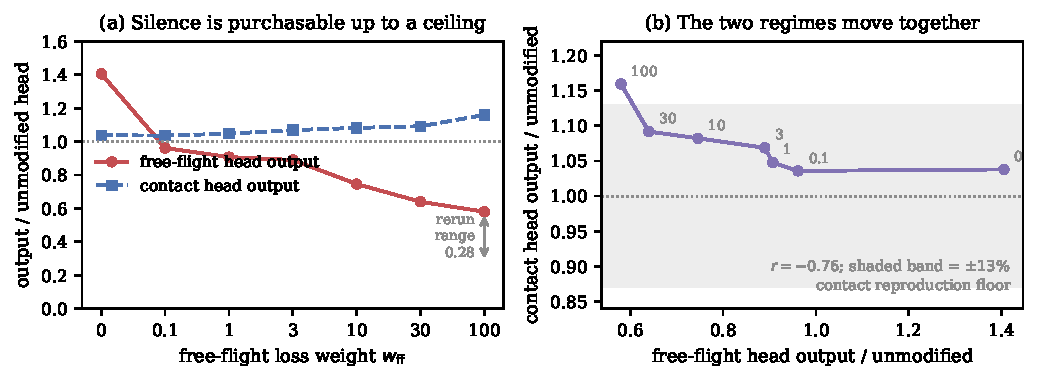
\includegraphics[width=0.62\textwidth]{figs/fig7_floor_ceiling.pdf}
\caption{The silence ceiling on frozen trunk features (exact-prior arm, seed 42;
the sweep is a refit of the residual head alone, so there is no seed spread to show).
Sweeping the free-flight window weight $w_{\text{ff}}$: free-flight head output falls
monotonically to $0.58$ of the unmodified head's value ($2.4\times$ of range) while
the contact-window head output drifts up $16\%$, so the two regimes move together
rather than trading off. Silence is not reachable on these features by weighting
alone. The dotted line is the unmodified head on the identical windows; the shaded
band in (b) is the measured contact reproduction floor of \S\ref{sec:limitations}, and
the arrow in (a) marks the range the endpoint takes when the same configuration is
rerun under a different random-number execution order ($0.28$--$0.58$).}
\label{fig:floor}
\end{figure}

\begin{table}[t]
\centering
\caption{The probe: supervision versus head output on free-flight windows (normalised RMS, position dimensions, seed 42).}
\label{tab:probe}
\small
\begin{tabular}{lcc}
\toprule
Arm & residual target RMS & head output RMS \\
\midrule
exact prior (Euler@.01$\times$5) & 0.0000 & 0.0197 \\
legacy prior (parabola)          & 0.0036 & 0.0203 \\
\bottomrule
\end{tabular}
\end{table}

\subsection{Reweighting buys one-step silence; an end-to-end gate starves}

The first intervention reweights the state loss on contact-flag-free windows (both the last input frame and the target frame contact-free) by a fixed $\times10$, chosen before the run. It works on the term it acts on: free-flight one-step error falls from 0.856 to 0.461\,px, the head's free-flight output RMS halves ($0.0186 \to 0.0095$; the single-seed probe reading in Table~\ref{tab:probe} is $0.0197$ for the same quantity on seed 42, a $6\%$ difference on a quantity whose reproduction difference is $0.5\%$), and---the part we did not expect---mixed error does not degrade ($0.570 \to 0.547$, a $4\%$ shift in the direction of improvement), so the contact regime paid nothing. Closed-loop free-flight error falls from 2.042 to 1.406 but misses its preregistered threshold (1.02). The second intervention adds a dedicated pathway: a per-sample gate between head and prior, trained end-to-end. It fails for a measurable reason. The regime mask is live on about 4.5\% of training windows (the stricter velocity-consistent subset that the evaluation scores is 0.4\%); the gradient that would teach the gate to close is outnumbered twenty to one, and the gate stays at its initialisation. Silence is purchasable with loss mass; a pathway alone is not.

\subsection{A supervised gate learns the regime but not the silence}

If starvation is the problem, supervise the gate directly: the regime label exists in the data as the contact flag, so we trained the gate with a binary cross-entropy against it, one preregistered arm. The gate learned the regime almost perfectly---99.34\% of windows, 95.5\% of free-flight windows closed. The silence did not follow: free-flight one-step error landed at 0.545\,px, closed-loop at 1.596, both worse than plain reweighting. The probe explains it. The gate is a soft attenuator---its mean on free-flight windows is 0.13 to 0.29, never zero---and the state loss constrains only the product of gate and residual. The head scaled its output up by $1.6$--$1.9\times$ to compensate, and the product, which is all that training sees, moved less than reweighting had moved it. Gate and head co-adapt. Two interventions, two lessons, one hypothesis forming: the loss geometry, rather than the architecture, may be the variable that matters here.

\subsection{Loss mass has a dose--response ceiling, and it reverses}

The third preregistration mapped the dose. Three arms held the exact prior and varied which loss term carried the extra mass: closed-loop loss $\times10$ (one-step untouched by design), both terms $\times10$, and single-step $\times100$. The two-component structure of the error shows up cleanly. Closed-loop mass attacks exactly the compounding term---closed-loop falls $24.9\%$ while the one-step free-flight error moves $1.8\%$ ($0.856 \to 0.872$, above the $0.5\%$ one-step reproduction floor) and mixed one-step rises $0.570 \to 0.602$, inside its preregistered 0.628\,px bound. Both terms together give the best closed-loop of the six treatment arms (Table~\ref{tab:arms}; $1.329$\,px) at a small one-step cost against its $\times10$ single-step reference (0.613 against 0.461\,px). And the single-step arm delivers the best free-flight one-step error of the study, 0.306\,px, while its closed-loop error \emph{reverses} to 2.727\,px---34\% worse than the unmodified baseline and 94\% worse than the $\times10$ arm it was derived from. The per-step profile is the mechanism: its error grows $2.6$--$3.9\times$ per feedback step and then $4.5$--$5.1\times$ on the next, in every seed, accelerating with depth, where no other arm's second-step growth exceeds $2.6\times$. Given enough single-step mass, the optimizer produced a head that is accurate once and unstable under its own feedback. We had the dose--response curve backwards in our preregistered expectation, and the reversal, not the improvement, is the finding: the two error components do not trade against each other monotonically, because the head is shared and the loss geometry overfits (Fig.~\ref{fig:dose}).

\subsection{Decode-time hard gating redeems the closed loop, at a quoted rate}

The four training-side interventions share a failure mode: they act through the shared head, so whatever they buy on free-flight windows is paid for on contact windows, and the exchange is not under control. The fifth intervention steps out of training entirely. At decode time, per rollout step, if the maximum contact-indicator probability over objects exceeds a threshold $\tau$, the head is used; below it, the head is skipped and the analytic prior acts alone. The threshold is selected on the first half of the validation windows (val-A), under a rule that bounds false silencing at $2\%$ of contact \emph{cells}, and all verdicts are computed on the second half (val-B).

The result closes the arc. Free-flight closed-loop error under the rule is $10^{-4}$\,px, in every seed, for the trained arms and for the unmodified baseline alike---parity with the analytic prior, from a trained model, with no retraining (Fig.~\ref{fig:roc}); \S\ref{sec:limitations} prices the one retrained copy, whose rule-selected threshold moves one grid step. Two qualifications keep the claim honest. The scored windows are few: the second validation half contains 15, 4 and 11 free-flight closed-loop windows across the three seeds, some thirty in all. The claim is therefore that the rule silenced every window it scored, and the residual transfer cost is small: across arms and seeds the val-B false-silence rate at the selected threshold runs $1.80$--$2.13\%$ of contact \emph{cells} (baseline arm: $1.92$--$2.01\%$), a mean of $1.96\%$ over the nine arm--seed pairs; the heavier evidence sits in the threshold scan that selects $\tau$ (22--26 free-flight windows per seed per threshold, and some 72{,}000 free-flight window-steps). The preregistered robustness readings for this slot confirm the mechanism directly: on the scored windows the all-silenced fraction is $1.0$ for all nine arm--seed pairs ($0.0$ with the rule disabled), and the per-window medians are $8.0$, $8.9$ and $9.2{\times}10^{-5}$\,px for seeds 42--44, identical across arms at fixed seed---once every window is silenced the prediction reduces to the analytic rollout, so the median records the prior floor read through the rule, not any property of a trained arm. A CPU recompute reproduces these readings to $10^{-7}$ relative (\texttt{S1f\_median\_recheck.json}). Nor does the rule redeem every arm: the dose-reversed $\times100$ arm's indicator inherits its degraded head, 4--22\% of its free-flight windows stay open at $\tau{=}0.9$, and the few open windows carry RMS 0.23--1.55\,px---silence presupposes a head whose errors are confined to the contact regime, and that arm no longer meets the premise. The indicator needs no training because it was always trained: the contact head's free-flight output probability is 0.040 on average against 0.973 on contact windows, and the $\tau$ rule merely reads it out. The cost is quoted with the same precision. The $2\%$ of contact \emph{cells} falsely silenced---$4.2$--$4.7\%$ of contact windows---lose the head's correction, and contact-regime closed-loop error rises by a factor of $1.12$--$1.21$ across arms, missing the $\times1.10$ tolerance we preregistered. A retrained copy of the baseline arm prices that band's stability: with the identical recipe and the same rule it selects $\tau^\ast{=}0.70$ instead of $0.75$ and reads $\times1.14$ instead of $\times1.21$---inside the original band, still above the $\times1.10$ tolerance, and $6\%$ away from its own first reading. Individual arm--seed points on this metric are not reproducible to better than about $6\%$. Appendix~\ref{app:silence_cost} closes that accounting per window, and shows why a two-percent rate is enough: the windows the rule silences are the high-error ones. Training the indicator for a better curve (two arms, preregistered) moved the protection rate by 0.8 percentage points---inside the reproduction floor of the metric it is read on---and left the curve where it was. One preregistered detail deviates in the shipped artifacts: the $\tau$ grid was registered at 0.50--0.99 in steps of 0.01 and shipped at 0.50--0.95 in steps of 0.05. An audit re-run at the registered resolution on the same split and rule (\texttt{S1f\_finegrid\_audit.json}) moves the landing point by at most 0.02 on every arm and seed ($\tau^\ast$: baseline 0.75, 0.80, 0.76; F1 0.86, 0.86, 0.87; F2 0.80, 0.82, 0.81), reaches the floor at every landing point (val-B all-silenced fraction $1.0$ on all nine pairs), and locates the first all-silenced threshold at 0.50--0.71, well below the landing point---so neither the landing point nor the floor is an artifact of the coarser grid. The same protocol, swept over every trained arm of the study, ships as Appendix~\ref{app:allarms}: the trade-off is unchanged, and the arms that miss the floor there are the ones whose indicator cannot confine its errors to the contact regime, as above.

\begin{figure}[t]
\centering
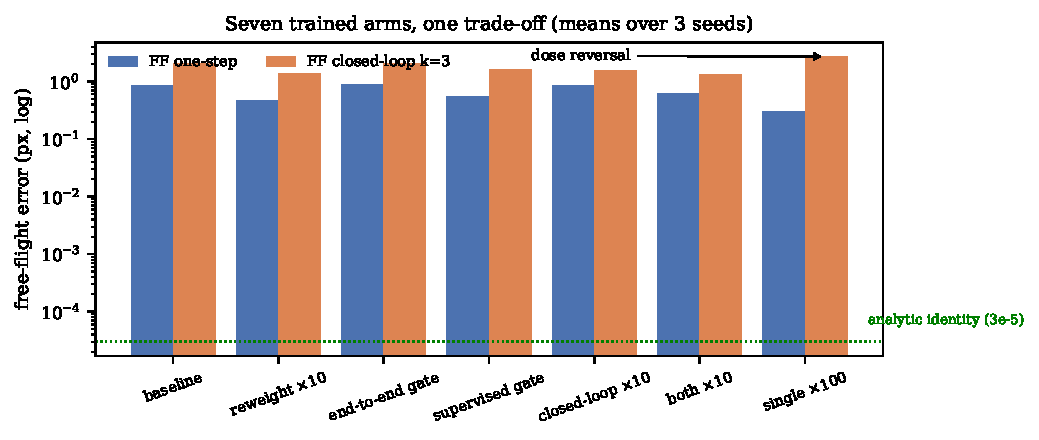
\includegraphics[width=\textwidth]{figs/fig4_dose_response.pdf}
\caption{All seven trained arms of Table~\ref{tab:arms} on the exact-prior branch, one trade-off. Free-flight one-step and closed-loop ($k{=}3$) errors, means over three seeds, log scale. The dotted line is the analytic identity ($3{\times}10^{-5}$\,px). The single-step arm achieves the best one-step error and the worst closed-loop error of the study.}
\label{fig:dose}
\end{figure}

\begin{figure}[t]
\centering
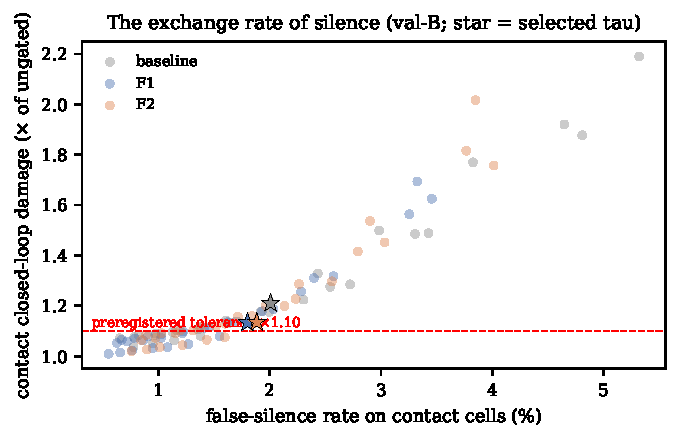
\includegraphics[width=0.62\textwidth]{figs/fig5_silence_roc.pdf}
\caption{The exchange rate of silence. Each point is one arm at one decode threshold $\tau$ (validation half); the $x$-axis is the false-silence rate on contact cells (\%) and the $y$-axis is contact-regime closed-loop damage relative to the same arm ungated. The three arms' curves coincide. Stars mark the preregistered selection rule's working points; the dashed line is the $\times1.10$ tolerance.}
\label{fig:roc}
\end{figure}

\subsection{One curve, one exchange rate}

Put the seven trained arms and the decode rule on one plot (Fig.~\ref{fig:dose}, Fig.~\ref{fig:roc}, and every arm's sweep in Fig.~\ref{fig:allarms}) and they do not scatter: they lie on a trade-off between free-flight silence and contact damage. Reweighting and the dose curve move along it from inside training; the decode rule reaches its far end from outside, by construction, and is the only point that achieves analytic parity at all. The exchange rate is the summary, and we give it as a measurement rather than an adjective: along the decode-rule scan, the false-silence percentage points paid per decade of free-flight closed-loop error purchased. On the baseline arm, moving $\tau$ from 0.5 to the silence floor buys 3.6--4.0 decades ($0.40$--$0.81$\,px down to $10^{-4}$\,px) for $0.55$--$1.23$ percentage points of cell-level false silence (per seed: 1.23, 0.71, 0.55---the floor arrives early where the indicator separates cleanly), a price of $0.15$--$0.31$ percentage points per decade (per seed: $0.31$, $0.18$, $0.15$); the preregistered operating point---the largest $\tau$ whose false-silence rate stays at or below $2\%$ of contact cells---sits at 1.9--2.0\% with the floor reached. From the unmasked baseline the whole purchase is 4.3 decades ($1.96 \to 10^{-4}$\,px). Both quantities are per-seed readings on a single scan; its threshold points share nested masks, so the across-seed spreads given above are the uncertainty we attach to them and no interval is placed on the slope. Whether a better regime indicator could shift the curve itself remains open---our one attempt moved it by less than the reproduction floor of the metric it is read on---but a practitioner choosing a deployment point no longer needs to guess the price.

\begin{figure}[t]
\centering
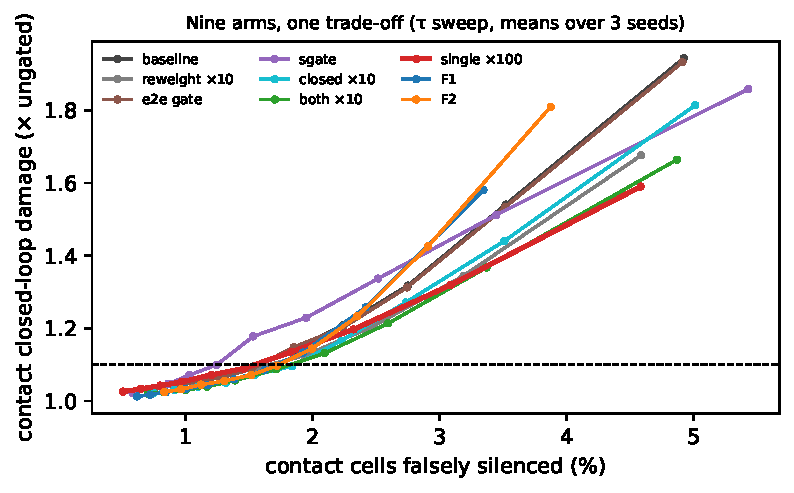
\includegraphics[width=0.62\textwidth]{figs/fig8_allarms_roc.pdf}
\caption{The threshold sweep for every trained arm of \S\ref{sec:silence}
under the protocol of Fig.~\ref{fig:roc} (means over three seeds; the red curve
is the single-step $\times100$ arm). The dashed line is the $\times1.10$ contact
tolerance. The three arms of \S\ref{sec:silence}'s report lie in this sweep and
reproduce its grid bit-identically.}
\label{fig:allarms}
\end{figure}

\begin{figure}[t]
\centering
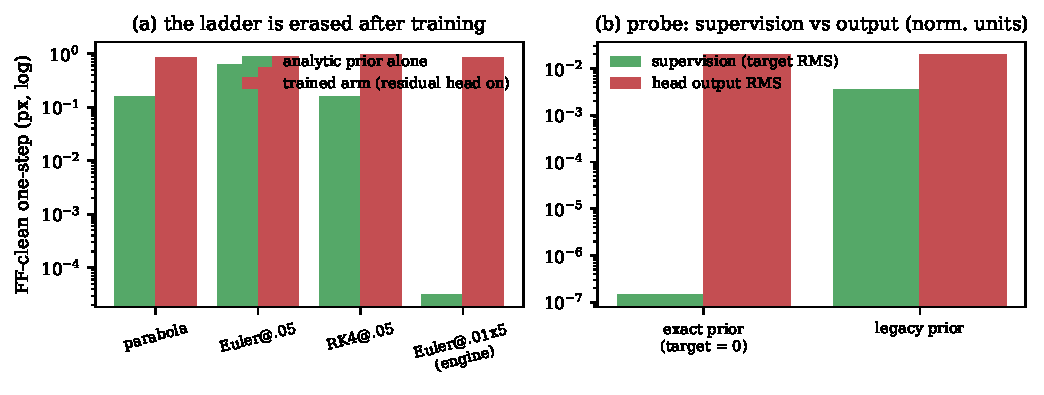
\includegraphics[width=\textwidth]{figs/fig3_interference.pdf}
\caption{(a) The analytic ladder (green) and the same arms after training (red) on free-flight windows: training erases the ladder. (b) The probe: on free-flight windows the exact-prior arm's supervision is $0.0000$ while its head outputs $0.0197$; the legacy arm's supervision matches its analytic prediction, and its head output is the same as the exact arm's.}
\label{fig:interference}
\end{figure}

\subsection{When the corrector is worth having}
\label{sec:when}

Everything above describes what the head costs on the windows where the prior is
already right. That raises the obvious question the paper would otherwise leave open:
is the head ever worth having? We can answer it, because the answer turns on the
\emph{kind} of mismatch rather than its size. Every prior in \S\ref{sec:floor} and
\S\ref{sec:silence} is wrong in the same way---through its discretisation, an error that
is per-window exact under a fixed substep and a constant action, and therefore leaves
nothing systematic to learn. We therefore varied the kind of mismatch while holding the
architecture, data budget, schedule and window convention fixed, and measured the head's
contribution under three priors: one that is numerically right, one whose gravity
parameter is wrong by $25\%$, and one that omits a drag and Coulomb-friction term
present in the data. The window convention, action index and metric follow
\S\ref{sec:platform}'s evaluation path and reproduce its published prior error to three
decimals ($0.0377$\,px against $0.038$).

\begin{table}[t]
\centering
\caption{The head's contribution as a function of what is wrong with the prior
(pendulum, seed 42, one run per cell, weighted position RMSE in px). ``Matched'' is the
control: the prior is numerically correct, and the head returns $-0.4\%$ in closed loop,
reproducing \S\ref{sec:silence}'s claim. Under a wrong parameter or an unmodelled force
the head removes $89$--$97\%$ of the closed-loop error it is handed. The last two rows
separate which part of the model does the work: freezing the trunk on \emph{matched}
data---so its hidden state cannot encode the mismatch---recovers almost all of the gain,
which places the contribution in the head rather than the trunk.}
\label{tab:corrector}
\small
\begin{tabular}{llccc}
\toprule
Condition & What is wrong with the prior & one-step (px) & closed $k{=}5$ (px) & $k{=}5$ gain \\
\midrule
prior & --- & 0.0377 & 0.4939 & --- \\
\quad + head & nothing (control) & 0.0428 & 0.4959 & $-0.4\%$ \\
\midrule
prior & gravity off by $25\%$ & 0.2123 & 5.0409 & --- \\
\quad + head & & 0.0516 & 0.5410 & $+89.3\%$ \\
\quad + head, frozen trunk & & 0.0443 & 0.3649 & $+92.8\%$ \\
\midrule
prior & unmodelled drag and friction & 0.2335 & 5.1126 & --- \\
\quad + head & & 0.0177 & 0.1569 & $+96.9\%$ \\
\quad + head, frozen trunk & & 0.0275 & 0.1905 & $+96.3\%$ \\
\bottomrule
\end{tabular}
\end{table}

Three things follow, and together they bound the paper's negative results. First, the
claim that the head is worthless is specific rather than general: it holds when the
prior's only error is its discretisation, and it reverses by an order of magnitude when
the prior is wrong in a way that is smooth, persistent and inferable from observations.
A reader should not conclude that residual correction is worthless; the correct
conclusion is that it is worth as much as the prior is wrong \emph{learnably}, and
nothing on the windows where the prior is already right. Second, the result is consistent with implicit parameter compensation by the head: in
the frozen-trunk ablation, a trunk fitted on matched data still permits most of the gain.
Because the cell is single-run and post-hoc, we do not claim this establishes online
identification as the mechanism. It places the result near classical identification work;
our measured contribution is the correction cost on windows where the prior is already right. Third, that ordering
has a practical consequence we did not expect: on the wrong-parameter prior, freezing
the trunk and adapting only the head is not merely as good as training both, it is
better, lowering closed-loop error from $0.488$ to $0.390$ over four seeds (a
$20.1\%$ reduction; equivalently, the full-trunk arm sits $25.4\%$ above the frozen
one, per-seed spread $6.2\%$, $t{=}8.2$, same direction on $4/4$). On the unmodelled-force
prior the same comparison gives $-3.5\%$ with an $18.3\%$ spread ($2/4$): no effect. So
we report it for the parameter-error case only, and read it as the trunk overfitting the
majority regime when it is allowed to keep training on data whose mismatch lives in the
minority windows.

One more measurement bears on the scope of the interference floor. In the contact-free pendulum, residual targets across four priors span about $100\times$. Re-evaluating each checkpoint on its own held-out split, the descriptive head-output/target ratios are $0.97 \pm 0.04$, $0.95 \pm 0.02$, $0.79 \pm 0.07$ and $0.126 \pm 0.008$ from the coarsest tier to the exact tier (Table~\ref{tab:ladder_extension}). This within-dataset sensitivity extension reuses the original three seeds and shares source trajectories; it is not an independent replication. The old shared-split values are retained in \texttt{m4\_floor\_partial.json} as an audit artifact only. Because most non-reference seeds' training sets overlap that validation set, we do not use its pooled-SD contrast as inferential evidence. The descriptive contrast remains: on this pendulum the trained head approximately scales with its residual target, whereas in the ball world the ratio spans $1.5$ to $1.4\times10^{5}$. The contrast is compatible with a regime-imbalance hypothesis: in the ball world, contact targets are near $0.015$ while free-flight targets are near $1.4\times10^{-7}$. These two worlds do not identify a universal threshold or establish that regime imbalance causally determines the floor.

Finally, we carried the decode rule into the matched-mismatch setting, since the
pendulum exposes an analogous contact channel through its phase head and is $88\%$ free
flight. The rule is monotonically harmful there: raising the threshold so that it
actually closes windows moves closed-loop error back toward the prior, from $0.541$
ungated to $0.586$ with every free-flight window silenced under the wrong-parameter
prior, and from $0.157$ to $0.262$ under the unmodelled force. The reason is the same
fact that makes the head useful above---when the head beats the prior in \emph{both}
regimes, a rule that silences it on one of them can only remove work. The gate is
therefore not a general improvement but a response to a specific condition, namely the
head being net harmful on the regime it silences; that condition is what this section
measures, and stating it as a condition rather than a technique is what we take to be
the transferable part.

\section{Structure and Recipe Cannot Substitute}\label{sec:substitute}

\subsection{The recipe multiplies within the floor}

The pendulum arms in \S\ref{sec:floor} were all trained single-step. If closed-loop failure is a training problem, a rollout loss should fix it. The preregistered answer took four arms across three recipe cells---single-step, closed-loop loss at the original learning rate, and closed-loop loss with the rate halved---and the gains track how unstable the arm was rather than how far it sat from the floor. The collapsing arm (pure GRU, closed-loop 53.89\,px) improves $41\times$ under the rollout loss; the coarse-prior arm improves $2.9\times$; the arm that was already stable---a strong MLP at 1.65\,px, $3.4\times$ above the exact arm's floor---gains nothing measurable (0\%, $t=-0.37$, $p=0.75$). That is the honest limit of the recipe: it repairs collapsing arms, and it does not reach the floor. The exact-prior arm was not run in the third cell, by preregistration, because there was nothing for the loss to act on. The best non-exact arm in any cell, 1.31\,px, remains $2.7\times$ above the exact arm's 0.49.

The cell design earned its keep by accident. The original two-cell plan (with the learning rate halved alongside the rollout loss) would have credited the loss for a degradation that belonged to the learning rate: single-step error rose in the halved-rate cell for every arm. The third cell separated the two, and the corrected reading---the rollout loss does not damage one-step accuracy at all---is one of the three self-corrections this protocol produced.

\subsection{Symbolic structure subtracts}

Symbolic structure has now been tested in this architecture family across four experiment generations: the 64-expert phase-gated arm (FiLM modulation of the residual head) in the unified main table, a ten-seed gating ablation and a capacity-decoupled block, and, in the ball world, the supervision $2\times2$ of the next paragraph. The four are not pooled into one sample: each is read through its own pairing, and Table~\ref{tab:c3} carries the per-generation estimates, intervals and pairing. The one quantity we do combine is a fixed-effect point estimate over the seven variants of the gating ablation, $+0.161$\,px; Table~\ref{tab:c3} gives its nominal interval ($[+0.116, +0.205]$), which we do not read as calibrated. The sign is positive in all seven, but only two of the seven individual intervals exclude zero (V1 $[+0.003, +0.316]$ and V2b $[+0.104, +0.309]$; V2c and V4 ran three of ten seeds), and the variants share seeds and training protocol, so we read the 7/7 sign count as one replicated finding rather than seven independent ones; a combined interval over the seven would assume independence and be anticonservative, so we quote only the nominal interval and do not read it as calibrated. Capacity is not matched across the gated/ungated pairs, and we state the deviation where the comparison is read: the gated arms replace the direct state head with the expert head, so the main table's gated arm carries $3.9\%$ fewer parameters than its control ($386{,}664$ vs $402{,}280$), the ablation's gated arms carry $8$--$16\%$ fewer for V1--V3 and Vfree and $17\%$ more for V4, and the capacity-decoupled block matches V3 to $0.1\%$ (Table~\ref{tab:c3}). The gating cost is therefore the cost of the gated head as implemented, not a capacity-matched effect. A routing audit shows that the gate leaves most of its experts unused (2 of 64 occupied in the decoupled variant, 9--15 of 64 in the fully coupled one). Two further cautions about numbers usually quoted for this result. The phase labels are themselves imbalanced---89\% of windows fall in three of eight classes and two classes never occur---and that histogram is identical for every arm, the ungated ones included, so it describes the data rather than the gate. And a free (unstructured) gate's difference from the structured ones is positive in point estimate but not distinguishable from zero ($+0.068$\,px, interval $[-0.069, +0.204]$), so we read it as giving no support to mis-chosen phase semantics as the culprit rather than as establishing equivalence. The full negative-result catalogue is in Appendix~\ref{app:negative}.

The $2\times2$ in Table~\ref{tab:p0c} separates the other channel, supervision, from capacity. Holding the architecture fixed and switching only loss weights, the label-supervised variants (C10, C11) are worse than the unsupervised ones (C00, C01) by 0.269\,px paired (95\% CI $[+0.096, +0.443]$, paired $t$ with 5 df), 6/6 seeds, $p=0.011$; the self-supervised prototype family contributes nothing measurable ($+0.022$\,px, CI $[-0.021, +0.065]$, 4/6 seeds). The supervision check confirms the mechanism was live---the supervised cells' indicator accuracy is 0.968 against 0.474 for the unsupervised cells---so the cost is paid by a head that demonstrably learned what we asked it to learn (Fig.~\ref{fig:p0c}). The reading we stand behind: phase labels are a description the state head does not need, and asking the trunk to predict them taxes the prediction we actually want.

\begin{table}[t]
\centering
\caption{Supervision $2\times2$ (ball world, six seeds, means). Architecture and capacity are identical across cells; only loss weights change.}
\label{tab:p0c}
\small
\begin{tabular}{lcccc}
\toprule
Cell & label supervision & prototype family & one-step (px) & closed-loop $k{=}5$ (px) \\
\midrule
C00 & off & off & \textbf{0.363} & \textbf{7.09} \\
C01 & off & on  & 0.393 & 7.99 \\
C10 & on  & off & 0.640 & 11.02 \\
C11 & on  & on  & 0.655 & 14.17 \\
\bottomrule
\end{tabular}
\end{table}

\subsection{The harm is absorbed by the floor}

One more experiment closes the $2\times2$'s logic. Run the exact-prior arm with symbolic structure attached and the harm disappears: at the exact tier, the gated variant lands within $0.0001$\,px of the ungated one (paired ratio $0.0005$)---a difference below the resolution of every other number in this paper, so the reading is that the harm becomes indistinguishable from zero, not that a small improvement was measured---while the gate's occupancy pathology is unchanged---the same handful of experts alive, the same dead classes (2--15 of 64 occupied depending on the variant; Table~\ref{tab:c3}). The structure still wastes capacity; the waste no longer costs anything, because the residual head has nothing to be wrong about. This is why the subtraction result and the floor result are one result: the harm of structure is a tax on the residual signal, and the residual signal is bounded by the floor.

\begin{figure}[t]
\centering
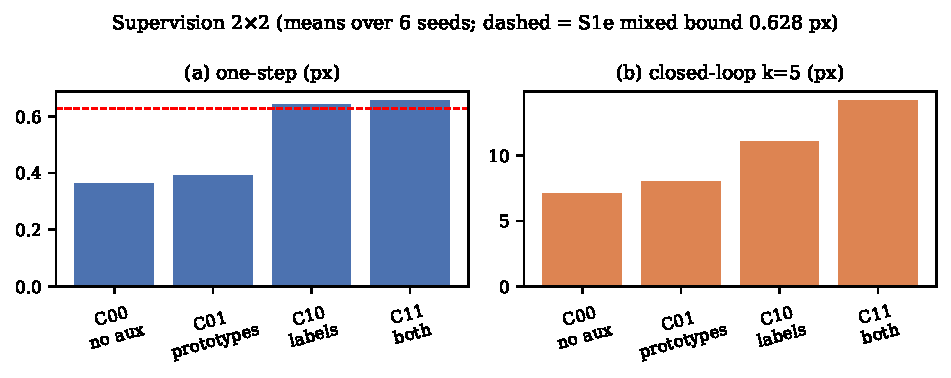
\includegraphics[width=0.82\textwidth]{figs/fig2_p0c_2x2.pdf}
\caption{Supervision $2{\times}2$ results (means over six seeds). Dashed line: the $0.628$\,px mixed-window contact-safety bound of the S1e preregistration quoted in \S\ref{sec:silence}---a reference point from a different experiment, not a criterion this $2\times2$ tested, since its own decision rule was a paired effect of $\pm0.23$\,px. Cells: C00 no auxiliary supervision, C01 prototypes only, C10 label supervision only, C11 both. (a)\ One-step error (px). (b)\ Closed-loop error at $k{=}5$ (px). The label-supervised cells (C10, C11) are consistently worse than the unsupervised ones (C00, C01).}
\label{fig:p0c}
\end{figure}



\section{Discussion}\label{sec:discussion}

\paragraph{A specification for hybrid deployment.} When a world model operates next to a simulator, the simulator's computation class---integrator, step size, and action sampling---should match the data-generating process at the scale being evaluated. Our identification experiment offers a caution, not a law. Under one registered Nelder--Mead protocol the fitted clean-world parameter lands about $22\%$ below the generating value, and nine starting values from $600$ to $1400$ converge to the same basin within $0.07\%$ (\S\ref{sec:basin}). That establishes stability of this local optimum under this protocol, not a global optimum, and we do not extend it to the regenerated worlds, which were not multi-started. In simulation, the generating integrator is knowable by code inspection or frame-level tests---our own preregistered analytic basis was wrong until the data corrected it (\S\ref{sec:platform}). With real sensor data there is no engine code to inspect, so identifying the computation class remains an open system-identification problem rather than a result demonstrated here.

\paragraph{Interference is not specific to this architecture.} We found the floor with a GRU residual head and mapped it with four training-side interventions and a decode-time gate, but the mechanism---a shared head trained on a regime-imbalanced mixture will not be silent on the minority regime---is a statement about loss geometry, and the balancing literature has met its cousins in other clothes \citep{lyle2021,metabalance2022}. The measured exchange rate is the part we believe generalises first: any proposal to make a residual head regime-quiet should be asked what it pays on the majority regime, in the currency of the metric that matters. We have staked the question, not the number: every measurement here comes from one architecture family in two planar worlds, and the exchange rate is what the next architecture should be asked to reproduce, not evidence that it will.

\paragraph{What remains of the symbolic programme.} Phase labels failed as gating signal, failed as supervision, and their occupancy pathology is structural. What survives is the audit use: the indicator that the decode rule reads is a trained phase head, and the occupancy table diagnosed the gating pathology before any accuracy number did. Cultural priors, in our experience, earn their place as instruments, not components. The filtering direction---maintaining beliefs over hidden states with an explicit computation-class prior---connects to Neural Bayesian Filtering~\citep{nbf2025}, which we defer to future work.

\paragraph{Discipline as an error-correction mechanism.} Three conclusions in this paper's history died inside the protocol: a gating advantage that was two negative arms compared to each other, a loss-quality claim that a third cell attributed to the learning rate, and a dose--response expectation that the reversal disproved. Each died cheaply, before publication, because the criteria were written first and the numbers had one source. We consider the protocol the second result of the paper.

\section{Limitations}\label{sec:limitations}

\textbf{Scale and domain.} Two simulated worlds---a two-link underactuated (acrobot) pendulum and a planar ball arena---with models between 339k and 615k parameters (\S\ref{sec:platform} breaks the range down by arm family). Every claim is scoped to these. The interference measurements and the optimizer-dependent parameter-compensation result are not tested at scale, in three dimensions, or on hardware; we make no general identification-law claim. Recurrent world models of this family remain competitive at the state of the art \citep{dreamerv3_2025}, which bounds how much of our conclusion is an artefact of model size.

\textbf{Sample size and the reproduction floor.} Trained comparisons use three to six seeds, paired. What we report is paired effects with confidence intervals (Tables~\ref{tab:p0c}, \ref{tab:c3}) and their direction across seeds. \citet{colas2018} show that a budget this small cannot support significance claims on small differences, and our own reproduction check is more specific than theirs. Retraining one arm from identical settings on the same hardware reproduces the analytic prior exactly ($0.00\%$), one-step error to $0.5\%$ and closed-loop $k{=}2$ to $0.2\%$, but its five-step closed-loop error moves from $14.07$ to $16.18$\,px---$15\%$, because the two runs select different best epochs, 35 and 59. That is the metric the ladder's second column is built on, and it is the least reproducible quantity we measured. The ball world prices the other axis: retraining its baseline arm under the identical recipe moves one-step error by $1.4\%$ and mixed closed-loop $k{=}3$ by $0.5\%$, but the decode rule's threshold selection moves one grid step ($0.75\to0.70$), the contact-damage reading moves $\times1.21\to\times1.14$ ($-6\%$), and the free-flight value at the selected threshold moves from $10^{-4}$ to $0.146$\,px---still inside the preregistered $0.20$\,px bound, but no longer at the prior floor. The floor is therefore metric-dependent as well as arm-dependent: across the ten seeds of the extension, the middle-tier trained arms carry cross-seed standard deviations of $0.8$--$3.2$\,px on this metric while the exact tier carries $0.008$\,px. We handle it by scope rather than by correction---the $29\times$ ball five-step ladder separation is the largest gap on the least reproducible metric; the pendulum closed-loop effects (a $20.1\%$ frozen-trunk reduction, a $24.9\%$ dose effect) and the $12$--$21\%$ contact damage are read on metrics whose reproduction floors we measured ($0.5$--$6\%$); the $34\%$ dose reversal is read on the ball $k{=}3$ free-flight metric; and decode-rule readings are quoted with their measured retraining spread ($6\%$ on the contact-damage ratio, one $\tau^\ast$ grid step, and $10^{-4}\to0.146$\,px on the free-flight value at the selected threshold)---and no rounding to four significant figures is load-bearing.

\textbf{The reproduction floor is two-dimensional.} The figures just quoted come from
retraining one arm at one seed, and they are the smaller of two axes. Evaluating ten
seeds of the same arm and recipe under the same protocol gives across-seed coefficients
of variation of $51\%$ (one-step), $12.6\%$ ($k{=}2$) and $16.4\%$ ($k{=}5$) at the coarse
tier, against the $0.5\%$, $0.2\%$ and $15\%$ that retraining moves the same three
quantities: on the two short metrics the seed axis is $69$--$100\times$ the retraining
axis, and on the five-step metric the two are comparable ($16\%$ against $15\%$).
Dropping the single most extreme seed leaves the coarse-tier one-step figure at $27\%$,
so this is a spread and not one outlier. Extending the ladder's coarse tier from three
seeds to ten moves its one-step mean from $0.97$ to $0.67$\,px (sd $0.34$), while the
exact tier stays at $0.038$\,px (sd $0.0006$, CV $1.7\%$)---an order of magnitude below
the other three tiers' $21$--$51\%$. The ladder's ordering and its $31\times$ closed-loop
separation survive this ten-seed extension: every one of the ten seeds is monotone in the
tier on both error columns. That is a within-sample robustness result, not an independent
replication---the extension reuses all three original seeds and adds seven---and its spread
includes split variation.
Two consequences follow. The design is paired everywhere for exactly this reason: a
same-seed comparison cancels the seed axis, which is why the $2\times2$ of
Table~\ref{tab:p0c} can resolve differences of a few per cent that an unpaired
comparison at this spread could not. And a diagnostic restriction of the measuring
stick---scoring every seed on one fixed validation split---halves the coarse-tier
dispersion ($51\%$ to $26\%$), but that split overlaps the other seeds' training data by
$88$--$91\%$, so it is a contaminated common-split sensitivity diagnostic and cannot estimate the
causal contribution of split variation; we do not use it as a noise-floor estimate.

\textbf{The silence line ends at a trade-off.} We did not achieve full closed-loop silence with training alone, and the one indicator-training attempt moved the ROC by less than the reproduction floor of the metric it is read on. The decode rule is a deployment answer with a quoted cost, not a training answer.

\textbf{Mechanism status.} The interference floor is measured, not derived, and
\S\ref{sec:flooranalysis} both removes three candidate explanations---representation
cost, loss mass, and a flat head on free-flight inputs---and identifies one term that
does counteract silence, the rollout loss. Two things stay open. The attainable
endpoint of the refit is underdetermined within roughly a factor of two: five refits
of one configuration, varying the random-number execution order and the training-pool
size, span $0.28$--$0.58$ of the unmodified head, so we quote a band and not a value.
And the representational component is inferred from repeated refits on one checkpoint
rather than measured as a property of the feature space, so we cannot say how much of
the floor is the trunk and how much is the objective. The subtraction result's cause
(why labels tax the trunk) is likewise unproven; we separated it from capacity and
measured its size.

\textbf{Scope of the interference-floor comparison.} In the contact-free pendulum, the own-split ten-seed mean ratios of head output to residual target are descriptively $0.126$--$0.968$ across four priors; the ball-world measurements span $1.5$ to $1.4\times10^{5}$ (\S\ref{sec:when}). The pendulum values are a within-dataset sensitivity extension with overlapping validation splits, not independent replications. Together the two worlds are consistent with a regime-imbalance hypothesis, but they do not identify a general regime boundary. We scope the measured interference-floor claim to the contact-rich setting and make no cross-world causal claim about its mechanism.

\textbf{The negative result about the corrector is scoped, not general.} Every claim in
this paper about the residual head being worthless comes from priors that are wrong only
through their discretisation, which is a per-window exact error and therefore leaves
nothing systematic to learn. \S\ref{sec:when} varies the kind of mismatch
instead of its magnitude and finds the head removing $89$--$97\%$ of the closed-loop
error when the prior's parameter is wrong or a force is missing
(Table~\ref{tab:corrector}), with the control
(matched prior) returning $-0.4\%$. A reader should take this paper's negative
results---and the interference floor in particular---as statements about what a learned
corrector costs on the regime where the prior is already right, not as evidence that it
is generally without value. \S\ref{sec:when} is post-hoc and single-run per
cell; we flag it here rather than in the body precisely because it scopes our own claims
and has not been through the protocol.

\textbf{Protocol scope.} Validation splits vary per seed (paired analysis only), windows-per-epoch was capped at 150k for cost, and the closed-loop evaluation window is five steps (pendulum) and three steps (ball)---short by design, since the pendulum's chaos saturates point predictions beyond it. The ball ladder's exact tier is exact only on the free-flight transfers that pass a velocity-consistency filter (6{,}597 of 64{,}463, about one in ten); on the unfiltered slice that tier is 0.4355\,px, $6\%$ better than the coarse tier rather than four orders of magnitude better, and on mixed windows it is $22\%$ worse. We report both slices in \S\ref{sec:floor} and claim float32-exactness only for the filtered one. The pendulum's exact tier is likewise not machine-exact: its 0.038\,px one-step floor is set by the intra-interval torque schedule that the 0.05\,s action labels do not record (0.018\,px on transition-free windows against 0.079\,px on the rest, \S\ref{sec:floor}); a full-observability control---the same protocol with the torque constant within each 0.05\,s interval---moves this floor to $3.0\times10^{-6}$\,px, confirming the attribution. The float32-exactness statement is scoped to the ball world, where the action schedule is fully observable. These spread estimates are descriptive, not a universal noise threshold: the repeated-run comparison uses one arm and one seed, while the R1 seed spread includes optimization and validation-split variation. The common-split R2 diagnostic reuses training episodes for most non-reference seeds and is not used to estimate a causal split effect. The decode rule's free-flight headline rests on only about thirty scored windows (\S\ref{sec:silence}).

\section{Reproducibility Statement}\label{sec:repro}

% TODO(C11): insert the public repository/archive URL or DOI before submission.
Artifact access: the released package is deposited at the archival URL recorded in the submission metadata (repository and DOI). The repository ships the two world generators with their validation suites, the full training and evaluation pipeline, and a manifest of 289 model checkpoints, each with a 16-character SHA-256 digest, across the 17 roots behind the claims here. It also ships twelve preregistration documents and 43 tests: prior-registry cross-implementation checks, document-to-JSON number consistency, checkpoint naming and overwrite protection, and architecture wiring assertions read back from state dictionaries. Every headline number in this paper is produced by a named script from a stored JSON in the analysis directory, and Appendix~\ref{app:provenance} lists the automated check that compares 319 of them against their sources, currently 319/319. The supplementary archive contains the manuscript sources, the twelve preregistrations with an English summary of every criterion they fix, the guard suite, the citation audit, and every stored JSON report quoted here; the trajectory datasets and model checkpoints (over 300\,MB) are excluded from the archive for size and are required by the training pipeline and by two of the provenance checks. All trained arms run on a single 8\,GB consumer GPU; the full experimental matrix is roughly forty GPU-hours. Preregistrations were committed before the first run of each of the twelve slots; \texttt{prereg\_manifest.json} records each file's SHA-256 digest and introduction commit beside the earliest commit of its slot's report artifacts (twelve of twelve precede or share the day of their first report). The gating series of \S\ref{sec:substitute} predates them and has no separate preregistration file in the release; its criteria, crash rule and both readings are carried in \texttt{E1a\_corrected\_report.json}, and we flag that as the one place where the paper reports an experiment whose criteria are documented only in its own analysis report. The two exceptions to strict pairing (per-seed validation splits, fixed identification windows) are declared in the preregistrations themselves. One preregistered detail deviates in the shipped artifacts: the SLOT-1f threshold grid was registered at 0.50--0.99 in steps of 0.01 and shipped at 0.50--0.95 in steps of 0.05; the registered-resolution audit is reported in \S\ref{sec:silence} (\texttt{S1f\_finegrid\_audit.json}). The floor analysis of \S\ref{sec:flooranalysis} is explicitly \emph{not} preregistered: it was run after the twelve slots, uses no new trained arms (it refits a head on frozen features from an existing checkpoint), and is reported as post-hoc mechanism work in a section that labels every claim it makes as measured or as an untested hypothesis.

\paragraph{Use of AI assistance.} Large language models were used for code drafting, prose editing, and literature retrieval under human direction. The experimental designs, preregistered criteria, and thresholds were specified by the authors; every quantitative claim is bound to a stored JSON by an executable guard script, and the guard suite (43 pytest tests plus 319 number-provenance checks) is part of the released artifacts.

\bibliographystyle{tmlr}
\bibliography{references}

\appendix

\section{Notation}\label{app:notation}
Four words carry more than one meaning in this paper. Table~\ref{tab:notation} fixes each sense used in the text, its unit, and where it is defined. Where a sentence gives a number without a unit, the unit is the one listed here.

\begin{table}[t]
\centering
\caption{Notation. ``Normalised RMS'' is the unit in which the head and target outputs are reported throughout the body; its scaling is defined below the table. ``px'' is the engine's native pixel unit.}
\label{tab:notation}
\small
\begin{tabular}{p{2.6cm}p{6.2cm}p{2.4cm}}
\toprule
Term & Meaning in this paper & Unit \\
\midrule
computation-class floor & The closed-loop error that a prior's computation class (equations and numerical scheme) sets, independent of any learned head. Measured by swapping the integrator (\S\ref{sec:floor}). & px \\
interference floor & The residual head's output on windows where the prior is already exact, set by the training mixture rather than by the prior (\S\ref{sec:silence}). & normalised RMS \\
silence (oracle) & A hard mask that zeroes the head on free-flight windows using the true contact flag. A diagnostic probe, not a deployable rule. & --- \\
silence (rule) & The deployed decode-time gate: the contact head's output probability thresholded at $\tau$ (\S\ref{sec:silence}). The only silence a model can run without oracle access. & --- \\
false silence & Fraction of contact \emph{cells} wrongly silenced by the rule; the body also reports the corresponding window-level fraction ($4.2$--$4.7\%$) (\S\ref{sec:silence}). & \% of contact cells \\
free-flight & Windows with no contact in the scored frames; the regime where the analytic prior is exact. & --- \\
analytic identity & The analytic prior's own closed-loop rollout, with no learned head; its error is the floor the decode rule reaches when every scored window is silenced. & px \\
prior tier & One integrator setting of the analytic prior (e.g.\ Euler@.05$\times$1, RK4@.01$\times$5). & --- \\
px vs.\ normalised & Position error in engine pixels versus head or target output in normalised units. The two are never compared directly. & px / norm. \\
\bottomrule
\end{tabular}
\end{table}

\paragraph{Normalised RMS, exactly.} A normalised residual is a difference of state vectors placed on unit scale: each dimension divided by its standard deviation over the training split. The prior, the target and the head output are all expressed in those units---the same ones the training loss operates in---and a ``normalised RMS'' is the root-mean-square of one such residual over a window set and the position dimensions: for $\mathcal{P}$ the position index set (six $(x,y)$ dimensions for the ball's three objects; four for the pendulum's two links) and $\mathcal{W}$ the windows (free-flight, where the body says so), $\bigl(|\mathcal{W}|^{-1}|\mathcal{P}|^{-1}\sum_{w\in\mathcal{W}}\sum_{d\in\mathcal{P}}\hat r_{w,d}^{2}\bigr)^{1/2}$. The mean over dimensions is unweighted---the training loss carries per-dimension weights, this diagnostic does not---and a normalised value is never converted to pixels: the conversion factor is per-dimension, so the two units are quoted side by side but never equated.

\section{Negative-result catalogue}\label{app:negative}
Table~\ref{tab:c3} gives the full accounting behind C5 for the gating generations---each comparison's pairing and the routing audit; the fourth generation, the supervision $2\times2$, is Table~\ref{tab:p0c}.
% AUTO-GENERATED by paper/tables/build_c3_table.py
\begin{table}[t]
\centering
\caption{The gating generations behind C5, with the pairing each
comparison actually uses; the fourth generation, the supervision $2\times2$,
is Table~\ref{tab:p0c}. $\Delta$ = (gated/supervised arm) $-$ (control arm) in
px, so $\Delta>0$ means the symbolic structure is worse; pairs share seeds and
validation splits. \emph{Occupied experts} is the number of expert groups that
receive non-zero routing mass (\texttt{gate\_fidelity.json}), min--max over runs.
Five caveats the table is built to expose: (i) the capacity-decoupled block is
paired against the coupled gated arm V3, \emph{not} against an ungated arm---no
paired ungated statistic for those arms is stored, so their unpaired means
(A1x64 0.753, A2x64 0.875, A3g1 0.904, against V3 0.877 and a 3-seed ungated
reference of 0.795) are not read as an advantage; (ii) the seven gating-ablation
variants share seeds and training protocol, so the fixed-effect combination is one
replicated finding, not seven independent ones, its $z$ is anticonservative, and
only 2 of the seven individual intervals exclude zero; (iii) the
phase-label histogram often quoted as an ``expert-occupancy audit''
(89\% of windows in three of eight classes, two classes never occurring) is
identical for every arm including the ungated ones (15 arms checked)---it
describes the data, not the gate; (iv) CIs are $t$-based; (v) capacity is not
matched across the gating pairs---the gated arms replace the direct state head
with an expert head, so the main-table gated arm carries 3.9\% fewer
parameters than its control ($386{,}664$ vs $402{,}280$), and the ablation's
gated arms carry 8--16\% fewer (V1--V3, Vfree) or 17\% more
(V4), while the capacity-decoupled block matches V3 to 0.1\%---so the gating
cost is the cost of the gated head as implemented, not a capacity-matched
effect.}
\label{tab:c3}
\footnotesize
\begin{tabular}{@{}p{2.15cm}p{4.15cm}rrrc@{}}
\toprule
Generation & Arm (paired against) & $\Delta$ (px) & 95\% CI & $n$ & Occupied experts \\
\midrule
main table & \texttt{ours\_gua} $-$ \texttt{ours\_base}, one-step & +0.272 & [+0.183, +0.362] & 3 & --- \\
 & \quad closed-loop $k{=}5$ & +27.181 & [-24.980, +79.342] & 3 & --- \\
\midrule
gating ablation ($\Delta$ = gated $-$ ungated) & V1 (4 experts) & +0.160 & [+0.003, +0.316] & 10 & 3--4 of 4 \\
 & V2a (16 experts) & +0.121 & [-0.079, +0.321] & 10 & 5--9 of 16 \\
 & V2b (16 experts) & +0.207 & [+0.104, +0.309] & 10 & 6--9 of 16 \\
 & V2c (16 experts) & +0.149 & [-0.057, +0.356] & 3 & 7--9 of 16 \\
 & V3 (64 experts) & +0.091 & [-0.087, +0.269] & 10 & 9--15 of 64 \\
 & V4 (256 experts) & +0.246 & [-0.010, +0.502] & 3 & 13--16 of 256 \\
 & Vfree (unstructured gate, 64 experts) & +0.068 & [-0.069, +0.204] & 10 & --- \\
 & \quad fixed-effect combination over the seven variants & +0.161 & [+0.116, +0.205] & 7 & --- \\
\midrule
capacity-decoupled ($\Delta$ = arm $-$ V3) & A1x64: supervise 1 axis, gate reads 1 & -0.099 & [-0.158, -0.040] & 6 & 2 of 64 \\
 & A3g1: supervise 3 axes, gate reads 1 & +0.038 & [-0.025, +0.100] & 5 & 2 of 64 \\
 & A2x64: supervise 2 axes, gate reads 2 & +0.066 & [-0.202, +0.334] & 6 & 6--8 of 64 \\
\bottomrule
\end{tabular}
\end{table}


The paper's claims are paired with the following preregistered negative results, reported at the same standard as the positive ones. Structure and supervision: symbolic gating (three gating generations; sign positive in all seven ablation variants, two individual intervals excluding zero; Table~\ref{tab:c3}); label supervision (2$\times$2, 6/6 negative); end-to-end gating (gradient starvation); supervised gating (co-adaptation). Loss geometry and identification: loss-mass dose (ceiling and reversal); indicator training (no ROC shift); single-step identification of parameters (compensation basin). Two further negatives are reported without a figure or table: confidence-gated source switching (no benefit) and multi-hypothesis prediction in a deterministic world (mode collapse). Table~\ref{tab:criteria} in Appendix~\ref{app:criteria} lists the criteria and their outcomes slot by slot, including the thresholds that missed; an English summary of every criterion accompanies the paper as \texttt{PREREG\_CRITERIA\_EN.md}, and crash accounting is in the preregistration files.

\paragraph{One pair of readings we report against ourselves.} The identification slot was first scored by an earlier criterion set that asked the clean-world estimate to land within $\pm20\%$ of the true value; it misses ($705.7$ against $900$, $21.6\%$ low), and the two companion criteria for the perturbed world (rollout recovery, and the parameter within $\pm20\%$ of $1125$) miss as well---three of six criteria, in all three seeds. The later preregistration of \S\ref{sec:floor} supersedes that criterion set by treating this fixed-start optimizer output as a replication target rather than as truth recovery; it passes $3/3$ under that target, while the earlier truth-recovery criteria fail. We report both readings, but do not treat the later pass as multi-start or optimizer-robust evidence. Per-seed verdicts for both sets are in the S2 identification reports.

\paragraph{A thesis test outside the twelve slots.} The G4 two-world shift test predates the twelve preregistrations of this paper and is not one of them. On a uniform $+25\%$ gravity shift it asked whether refitting the prior beats leaving it fixed; in no seed does it: the fixed prior's $k{=}5$ error is $5.10/5.32/5.36$\,px against the refitted prior's $5.99/6.08/6.33$\,px, and four of its five recorded criteria---net benefit, prior-as-liability, in-class identification, out-of-class extension---read false in every seed (\texttt{S2\_g4\_s\{42,43,44\}.json}), with only the architecture criterion passing. We reproduce the false verdicts here rather than quote the single pass.




\section{Provenance check}\label{app:provenance}
The automated provenance check compares 319 numbers quoted in this paper against their source JSON reports (tolerances per number). Current status: 319/319 PASS. The check script and its output are part of the release; any edits to the paper's numbers must re-run it.
% AUTO-GENERATED by paper/tables/gen_provenance.py (v3, unicode-safe)
% from analysis_output/number_provenance_check.json
% 319 checks, generated from analysis_output/number_provenance_check.json
{\small
\begin{tabular}{p{8.2cm}rrc}
\toprule
Check & computed & quoted & status \\
\midrule
E0 ours\_base@rk4001x5 one-step & 0.036981 & 0.037 & PASS \\
E0 ours\_base@rk4001x5 closed k=5 & 0.492429 & 0.49 & PASS \\
E0 ladder coarse one-step & 0.969015 & 0.969 & PASS \\
E0 ladder coarse closed k=5 & 14.2577 & 14.26 & PASS \\
E0 analytic exact one-step & 0.037827 & 0.038 & PASS \\
E0 analytic coarse one-step & 3.37273 & 3.373 & PASS \\
pendulum ramp-window fraction & 0.1876 & 0.188 & PASS \\
pendulum exact tier one-step, da=0 (px) & 0.017665 & 0.018 & PASS \\
pendulum exact tier one-step, da!=0 (px) & 0.079238 & 0.079 & PASS \\
pendulum exact tier granularity gap (px) & 0.061573 & 0.06 & PASS \\
pendulum exact tier one-step overall (px) & 0.037834 & 0.038 & PASS \\
pendulum obsgrid prior one-step (px) & 3e-06 & 3e-06 & PASS \\
pendulum obsgrid trained arm one-step (px) & 0.000248 & 0.00025 & PASS \\
pendulum obsgrid arm vs plateau ratio & 152.712 & 150 & PASS \\
ball repro one-step rel diff (\%) & 1.36509 & 1.4 & PASS \\
ball repro mixed k=3 rel diff (\%) & 0.502688 & 0.5 & PASS \\
ball repro contact damage at tau* & 1.13623 & 1.14 & PASS \\
ball repro contact damage rel diff (\%) & 6.11867 & 6 & PASS \\
ball repro rule-selected tau* & 0.7 & 0.7 & PASS \\
ball repro free-flight at tau* (px) & 0.145947 & 0.146 & PASS \\
ball ladder parabola FF-clean & 0.159111 & 0.1591 & PASS \\
ball ladder euler005 FF-clean & 0.636397 & 0.6364 & PASS \\
ball ladder exact FF-clean & 3.1e-05 & 3e-05 & PASS \\
ball ladder exact FF-unfiltered & 0.435489 & 0.4355 & PASS \\
ball ladder coarse FF-unfiltered & 0.464663 & 0.4647 & PASS \\
ball ladder exact/coarse ratio, unfiltered & 0.937216 & 0.937 & PASS \\
ball unfiltered exact-vs-coarse improvement (\%) & 6.27838 & 6 & PASS \\
ball filter retention (n\_ff\_clean/n\_ff) & 0.102338 & 0.1023 & PASS \\
ball mixed windows: exact tier (px) & 1.1071 & 1.1071 & PASS \\
ball mixed windows: coarse tier (px) & 0.904906 & 0.9049 & PASS \\
ball mixed windows: exact/coarse penalty & 1.22344 & 1.224 & PASS \\
S1g wff0 head RMS (normalised) & 0.021259 & 0.0213 & PASS \\
S1g same-seed baseline head RMS & 0.019673 & 0.0197 & PASS \\
S1g wff0 vs same-seed baseline (\%) & 8.05873 & 8 & PASS \\
S1g wff10 head RMS (seed 42) & 0.008872 & 0.0089 & PASS \\
S1c baseline head RMS (3-seed mean) & 0.018574 & 0.0186 & PASS \\
S1c wff10 head RMS (3-seed mean) & 0.009493 & 0.0095 & PASS \\
S1g wff0 vs 3-seed baseline mean (\%) & 14.4551 & 14 & PASS \\
ff Jacobian norm, exact-prior arm (mean) & 0.660329 & 0.66 & PASS \\
ff Jacobian norm, six-arm mean & 0.888982 & 0.89 & PASS \\
contact Jacobian norm, mean & 0.42945 & 0.43 & PASS \\
P0b noprior A k=5 & 53.8913 & 53.89 & PASS \\
P0b noprior C k=5 & 1.31263 & 1.31 & PASS \\
P0b exact A k=5 & 0.49407 & 0.49 & PASS \\
P0c C00 one-step & 0.363424 & 0.363 & PASS \\
P0c C10 one-step & 0.639984 & 0.64 & PASS \\
P0c yao main effect & 0.269474 & 0.269 & PASS \\
S0b absorption ratio & 0.000508 & 0.0005 & PASS \\
S0b delta one-step & 0.000138 & 0.0001 & PASS \\
S1b exact-arm FF (trained) & 0.861268 & 0.861 & PASS \\
S1c baseline FF (via S1e) & 0.855817 & 0.856 & PASS \\
S1c wff10 FF & 0.46092 & 0.461 & PASS \\
S1e W-arm one-step FF (x100) & 0.306251 & 0.306 & PASS \\
S1e W-arm closed k=3 (x100) & 2.72681 & 2.727 & PASS \\
S1d gate accuracy & 0.9934 & 0.9934 & PASS \\
S1f decode-rule FF closed (max over arms/seeds) & 0.000103 & 0.0001 & PASS \\
S1f false-silence at tau* & 0.019575 & 0.02 & PASS \\
S1f val-B FF median, seed 42 (1e-5 px) & 8.02599 & 8 & PASS \\
S1f val-B FF median, seed 43 (1e-5 px) & 8.94829 & 8.9 & PASS \\
S1f val-B FF median, seed 44 (1e-5 px) & 9.2449 & 9.2 & PASS \\
S1f val-B FF median spread across arms (px) & 0 & 0 & PASS \\
S1f val-B all-silenced fraction at tau* (min, 9 pairs) & 1 & 1 & PASS \\
S1f unmasked all-silenced fraction (max, 9 pairs) & 0 & 0 & PASS \\
S1f CPU-recheck max relative deviation & 0 & 1e-07 & PASS \\
S1f finegrid tau* shift (max |d|, all 9 pairs) & 0.02 & 0.02 & PASS \\
S1f finegrid val-B all-silenced at tau* (min, 9 pairs) & 1 & 1 & PASS \\
S1f finegrid first all-silenced tau (min) & 0.5 & 0.5 & PASS \\
S1f finegrid first all-silenced tau (max) & 0.71 & 0.71 & PASS \\
S1f allarms arms (n) & 9 & 9 & PASS \\
S1f allarms vs report grid (max rel diff, shared arms) & 0 & 0 & PASS \\
S1f allarms tau* (min) & 0.75 & 0.75 & PASS \\
S1f allarms tau* (max) & 0.85 & 0.85 & PASS \\
S1f allarms contact damage at tau* (min) & 1.08354 & 1.08 & PASS \\
S1f allarms contact damage at tau* (max) & 1.29197 & 1.29 & PASS \\
S1f allarms damage at tau=0.5 (min) & 1.01253 & 1.01 & PASS \\
S1f allarms damage at tau=0.5 (max) & 1.03622 & 1.04 & PASS \\
S1f allarms damage at tau=0.95 (min) & 1.58105 & 1.58 & PASS \\
S1f allarms damage at tau=0.95 (max) & 1.94396 & 1.94 & PASS \\
S1f allarms arm-seeds reaching floor at tau* (n) & 22 & 22 & PASS \\
S1f allarms S-arm all-silenced (max) & 0.75 & 0.75 & PASS \\
S1f allarms S-arm FF at tau* (min, px) & 0.577686 & 0.58 & PASS \\
S1f allarms S-arm FF at tau* (max, px) & 2.07441 & 2.07 & PASS \\
S2 clean g (identical across 3 seeds) & 705.733 & 705.7 & PASS \\
S2 g125 H5 g (min) & 870.87 & 870.9 & PASS \\
S2 g125 H5 g (max) & 886.448 & 886.4 & PASS \\
S2 g125 H5 spread (\%) & 1.78879 & 1.8 & PASS \\
S2 refined g (min) & 957.3 & 957.3 & PASS \\
S2 refined g (max) & 961.392 & 961.4 & PASS \\
S2 refined spread (\%) & 0.427399 & 0.4 & PASS \\
S2 horizon monotone H1<H5<H10 (all seeds) & 1 & 1 & PASS \\
G4 s42 fixed prior k=5 (px) & 5.10275 & 5.1 & PASS \\
G4 s42 refitted prior k=5 (px) & 5.98858 & 5.99 & PASS \\
G4 s42 criteria A-D all false & 0 & 0 & PASS \\
G4 s42 criterion E true & 1 & 1 & PASS \\
G4 s43 fixed prior k=5 (px) & 5.32375 & 5.32 & PASS \\
G4 s43 refitted prior k=5 (px) & 6.07538 & 6.08 & PASS \\
G4 s43 criteria A-D all false & 0 & 0 & PASS \\
G4 s43 criterion E true & 1 & 1 & PASS \\
G4 s44 fixed prior k=5 (px) & 5.36179 & 5.36 & PASS \\
G4 s44 refitted prior k=5 (px) & 6.32649 & 6.33 & PASS \\
G4 s44 criteria A-D all false & 0 & 0 & PASS \\
G4 s44 criterion E true & 1 & 1 & PASS \\
E0 euler001x5 roll5 seed-std & 2.43455 & 2.43 & PASS \\
E0 rk4005 roll5 seed-std & 1.3332 & 1.33 & PASS \\
E0 exact roll5 seed-std & 0.009343 & 0.01 & PASS \\
E0 analytic prior roll5 spread (x) & 31.9338 & 32 & PASS \\
E0 trained-arm roll5 spread (x) & 28.9537 & 29 & PASS \\
E0 head contribution coarse (improve) & 0.097836 & 0.098 & PASS \\
E0 head contribution euler001x5 (degrade) & 0.50339 & 0.504 & PASS \\
ball parabola = 0.225/sqrt2 & 0.159111 & 0.159099 & PASS \\
ball euler005 = 0.9/sqrt2 & 0.636397 & 0.636396 & PASS \\
ball exact closed-loop k=5 (1.4e-4) & 0.000138 & 0.000138 & PASS \\
P0b coarse improvement (x) & 2.89249 & 2.9 & PASS \\
P0b stable-arm improvement (x) & 1.00261 & 1 & PASS \\
training win\_ff fraction & 0.045055 & 0.045 & PASS \\
eval ff\_clean fraction & 0.003683 & 0.004 & PASS \\
S1e W1 one-step FF & 0.871577 & 0.872 & PASS \\
S1e W1 one-step mixed & 0.601986 & 0.602 & PASS \\
S1e W1 closed k=3 FF & 1.53338 & 1.533 & PASS \\
S1e W1 closed-loop fall & 0.248987 & 0.249 & PASS \\
S1e W2 one-step FF & 0.612884 & 0.613 & PASS \\
S1e S step1 growth (min) & 2.63228 & 2.63 & PASS \\
S1e S step1 growth (max) & 3.93032 & 3.93 & PASS \\
S1e S step2 growth (min) & 4.54704 & 4.55 & PASS \\
S1e S step2 growth (max) & 5.08212 & 5.08 & PASS \\
S1e others step2 growth (max) & 2.5456 & 2.55 & PASS \\
S1f val-B FF windows (15/4/11) & 10 & exactly [15, 4, 11] & PASS \\
S1f scan FF windows per seed/tau (range) & 5 & n in [22, 26] across seeds/tau & PASS \\
S1f S-arm win|0.9 ff rms (min) & 0.229276 & 0.23 & PASS \\
S1f S-arm win|0.9 ff rms (max) & 1.54625 & 1.55 & PASS \\
S1f S-arm open fraction at 0.9 (min) & 0.038462 & 0.04 & PASS \\
S1f S-arm open fraction at 0.9 (max) & 0.217391 & 0.22 & PASS \\
S1f baseline floor dfs pp (min) & 0.551276 & 0.55 & PASS \\
S1f baseline floor dfs pp (max) & 1.23072 & 1.23 & PASS \\
S1f baseline floor decades (min) & 3.59811 & 3.6 & PASS \\
S1f baseline floor decades (max) & 4.01243 & 4.01 & PASS \\
S1f operating-point fs\% (mean) & 1.97286 & 1.97 & PASS \\
S1f unmasked-to-floor decades & 4.2923 & 4.3 & PASS \\
S1f val-B false-silence min (9 pairs, \%) & 1.79975 & 1.8 & PASS \\
S1f val-B false-silence max (9 pairs, \%) & 2.13272 & 2.13 & PASS \\
S1f val-B false-silence baseline min (\%) & 1.9174 & 1.92 & PASS \\
S1f val-B false-silence baseline max (\%) & 2.00734 & 2.01 & PASS \\
S1f val-B false-silence mean (9 pairs, \%) & 1.9626 & 1.96 & PASS \\
S1f tau=0.5 baseline FF min (px) & 0.395501 & 0.4 & PASS \\
S1f tau=0.5 baseline FF max (px) & 0.808829 & 0.81 & PASS \\
S1f unmasked baseline FF (mean, px) & 1.96085 & 1.96 & PASS \\
S1f indicator free-cell prob (k=1 mean) & 0.038917 & 0.04 & PASS \\
S1f indicator contact-cell prob (k=1 mean) & 0.973165 & 0.973 & PASS \\
P0c main-effect CI half-width (t, df=5) & 0.173751 & 0.174 & PASS \\
P0c main-effect CI lower (t) & 0.095723 & 0.096 & PASS \\
P0c main-effect CI upper (t) & 0.443225 & 0.443 & PASS \\
P0c prototype effect & 0.022015 & 0.022 & PASS \\
P0c prototype CI lower (t) & -0.020976 & -0.021 & PASS \\
P0c prototype CI upper (t) & 0.065005 & 0.065 & PASS \\
gate meta pooled effect (px) & 0.160514 & 0.161 & PASS \\
C3 gen2 individual CIs excluding zero (count) & 2 & 2 & PASS \\
C3 V1 individual CI low (px) & 0.003171 & 0.003 & PASS \\
C3 V2b individual CI low (px) & 0.104395 & 0.104 & PASS \\
C3 Vfree delta (px) & 0.0677 & 0.068 & PASS \\
C3 Vfree CI low (px) & -0.069062 & -0.069 & PASS \\
C3 Vfree CI high (px) & 0.204462 & 0.204 & PASS \\
C3 main-table gated params (k) & 386.664 & 386.664 & PASS \\
C3 main-table control params (k) & 402.28 & 402.28 & PASS \\
C3 main-table capacity deviation (\%) & -3.88 & -3.9 & PASS \\
C3 ablation fewer-capacity range min (\%) & 7.97 & 8 & PASS \\
C3 ablation fewer-capacity range max (\%) & 15.71 & 16 & PASS \\
C3 V4 capacity deviation (\%) & 16.8 & 17 & PASS \\
C3 decoupled capacity deviation (max, \%) & 0.07 & 0.1 & PASS \\
S1f exchange rate (min pp/decade) & 0.153213 & 0.153 & PASS \\
S1f exchange rate (max pp/decade) & 0.306728 & 0.307 & PASS \\
crash rate: five slots (sum) & 0 & 0 & PASS \\
crash rate: P0c 2x2 (0/24) & 0 & 0 & PASS \\
manifest checkpoints (n) & 289 & 289 & PASS \\
reported model sizes (min, k params) & 339.076 & 339 & PASS \\
reported model sizes (max, k params) & 615.158 & 615 & PASS \\
pendulum model sizes (max, k params) & 431.305 & 431 & PASS \\
capacity ablations (max, k params) & 469.864 & 470 & PASS \\
silence hist: silenced with-head RMS (min) & 7.59349 & 7.6 & PASS \\
silence hist: silenced with-head RMS (max) & 8.72092 & 8.7 & PASS \\
silence hist: silenced skipped-head RMS (min) & 9.73095 & 9.7 & PASS \\
silence hist: silenced skipped-head RMS (max) & 10.7051 & 10.7 & PASS \\
silence hist: contact pool RMS (max) & 2.28184 & 2.3 & PASS \\
silence hist: windows touched by rule (min, \%) & 4.19953 & 4.2 & PASS \\
silence hist: windows touched by rule (max, \%) & 4.66007 & 4.7 & PASS \\
silence hist: identity residual (max) & 1e-06 & 0 & PASS \\
S1c reweighting R3 (closed-loop) fails & 1 & 1 & PASS \\
S1d supervised gate R3d (closed-loop) fails & 1 & 1 & PASS \\
S1f R2f contact-safety fails (9/9 arm-seed) & 1 & 1 & PASS \\
S2 preregistered R2-a/b/c all pass & 1 & 1 & PASS \\
S1e main criterion R3e fails on every arm & 1 & 1 & PASS \\
floor exact clean-FF head RMS & 0.019673 & 0.0197 & PASS \\
floor legacy clean-FF head RMS & 0.020264 & 0.0203 & PASS \\
floor prior spread across four tiers (x) & 1.21959 & 1.22 & PASS \\
floor coarse vs exact head RMS (z) & 2.67523 & 2.68 & PASS \\
floor within-prior seed CV (\%) & 8.24243 & 8.2 & PASS \\
floor ceiling w\_ff=100 (corrected head) & 0.579755 & 0.58 & PASS \\
floor ceiling dynamic range (x) & 2.42446 & 2.42 & PASS \\
floor ceiling monotone in w\_ff & 1 & 1 & PASS \\
floor ceiling contact max deviation (\%) & 15.9528 & 16 & PASS \\
floor rollout at matched fit (x) & 1.61654 & 1.62 & PASS \\
floor rollout matched no-roll Huber & 0.00269 & 0.00269 & PASS \\
floor rollout matched roll Huber & 0.00256 & 0.00256 & PASS \\
floor rollout contrast (x) & 4.71445 & 4.71 & PASS \\
floor rerun spread max (x) & 0.579755 & 0.58 & PASS \\
floor rerun spread min (x) & 0.277979 & 0.278 & PASS \\
floor sample-size effect 120k/400k (x) & 1.07464 & 1.07 & PASS \\
floor rollout contrast 120k matched (x) & 2.74919 & 2.75 & PASS \\
floor free-trunk plateau & 0.470319 & 0.47 & PASS \\
floor free-trunk contact improvement & 0.920125 & 0.92 & PASS \\
floor pooled no-roll band (min) & 0.277979 & 0.28 & PASS \\
floor pooled no-roll band (max) & 0.579755 & 0.58 & PASS \\
S1c reweighted / baseline (FF one-step) & 0.538573 & 0.54 & PASS \\
S1e single-step x100 / baseline (FF one-step) & 0.357846 & 0.36 & PASS \\
frozen w\_ff=10 / unmodified & 0.745785 & 0.75 & PASS \\
frozen w\_ff=0 / unmodified & 1.40559 & 1.41 & PASS \\
original head Huber on same features & 0.007172 & 0.0072 & PASS \\
E5 matched head gain k=5 (\%) & -0.419872 & -0.4 & PASS \\
E5 g1125 prior one-step (px) & 0.212332 & 0.2123 & PASS \\
E5 g1125 head gain k=5 (\%) & 89.2679 & 89.3 & PASS \\
E5 drag prior one-step (px) & 0.233533 & 0.2335 & PASS \\
E5 drag head gain k=5 (\%) & 96.9308 & 96.9 & PASS \\
E5-M2 g1125 frozen-trunk gain k=5 (\%) & 92.7619 & 92.8 & PASS \\
E5-M2 drag frozen-trunk gain k=5 (\%) & 96.2738 & 96.3 & PASS \\
E5-M2c g1125 ungated k5 (px) & 0.548433 & 0.548 & PASS \\
E5-M2c g1125 all-closed k5 (px) & 0.585775 & 0.586 & PASS \\
E5-M2c drag ungated k5 (px) & 0.156915 & 0.157 & PASS \\
E5-M2c drag all-closed k5 (px) & 0.262085 & 0.262 & PASS \\
legacy common-split exact ratio, seed 42 (audit only) & 0.113933 & 0.11 & PASS \\
own-split floor ratio euler005 descriptive mean & 0.968258 & 0.968 & PASS \\
own-split floor ratio euler005 descriptive SD & 0.042795 & 0.043 & PASS \\
own-split floor ratio euler001x5 descriptive mean & 0.95281 & 0.953 & PASS \\
own-split floor ratio euler001x5 descriptive SD & 0.023693 & 0.024 & PASS \\
own-split floor ratio rk4005 descriptive mean & 0.791798 & 0.792 & PASS \\
own-split floor ratio rk4005 descriptive SD & 0.06973 & 0.07 & PASS \\
own-split floor ratio rk4001x5 descriptive mean & 0.125863 & 0.126 & PASS \\
own-split floor ratio rk4001x5 descriptive SD & 0.008239 & 0.008 & PASS \\
own-split floor ratio uses ten seeds & 1 & 1 & PASS \\
own-split floor ratio reports descriptive-only status & 1 & 1 & PASS \\
own-split floor ratio does not claim inferential gap & 1 & 1 & PASS \\
pendulum head\_ff across 4 priors (max/min) & 830.35 & 830 & PASS \\
M4 g1125 full over frozen inflation (\%) & 25.4385 & 25.4 & PASS \\
M4 g1125 frozen-vs-full reduction (\%) & 20.1204 & 20.1 & PASS \\
M4 g1125 per-seed spread (\%) & 6.22454 & 6.2 & PASS \\
M4 g1125 full mean (px) & 0.487718 & 0.488 & PASS \\
M4 g1125 frozen mean (px) & 0.389587 & 0.39 & PASS \\
M4 drag improvement (\%) & -3.50499 & -3.5 & PASS \\
M4 drag per-seed spread (\%) & 18.2953 & 18.3 & PASS \\
M4 seed variation one-step CV (\%) & 4.48294 & 4.5 & PASS \\
M4 floor ratio coarse (mean) & 0.981081 & 0.98 & PASS \\
M4 floor ratio coarse (sd) & 0.016072 & 0.02 & PASS \\
M4 floor ratio exact (mean) & 0.125273 & 0.13 & PASS \\
M4 floor ratio exact (sd) & 0.008118 & 0.008 & PASS \\
M4 floor ratio euler001x5 (mean) & 0.957675 & 0.96 & PASS \\
M4 floor ratio euler001x5 (sd) & 0.008985 & 0.01 & PASS \\
M4 floor ratio rk4005 (mean) & 0.696929 & 0.7 & PASS \\
M4 floor ratio rk4005 (sd) & 0.091716 & 0.09 & PASS \\
M4 all four tiers have n=7 & 1 & 1 & PASS \\
M4 floor separation z (exact vs coarse) & 47.5305 & 47.5 & PASS \\
noise floor coarse one-step seed CV (\%) & 50.9539 & 51 & PASS \\
noise floor coarse k=2 seed CV (\%) & 12.5481 & 12.6 & PASS \\
noise floor coarse k=5 seed CV (\%) & 16.4363 & 16.4 & PASS \\
noise floor retrain one-step (\%) & 0.511496 & 0.51 & PASS \\
noise floor retrain k=2 (\%) & 0.181491 & 0.18 & PASS \\
noise floor retrain k=5 (\%) & 14.9567 & 14.96 & PASS \\
noise floor seed/retrain ratio one-step & 99.6174 & 100 & PASS \\
noise floor seed/retrain ratio k=2 & 69.1392 & 69 & PASS \\
noise floor seed/retrain ratio k=5 & 1.09892 & 1.1 & PASS \\
noise floor coarse one-step LOO CV (\%) & 27.2279 & 27 & PASS \\
noise floor coarse one-step ten-seed mean (px) & 0.66521 & 0.67 & PASS \\
noise floor coarse one-step ten-seed sd (px) & 0.33895 & 0.34 & PASS \\
noise floor exact one-step ten-seed mean (px) & 0.037521 & 0.038 & PASS \\
noise floor exact one-step ten-seed sd (px) & 0.000629 & 0.0006 & PASS \\
noise floor exact one-step CV (\%) & 1.67759 & 1.7 & PASS \\
noise floor 10-seed k=5 ladder separation (x) & 30.9776 & 31 & PASS \\
noise floor matrix covers ten seeds & 1 & 1 & PASS \\
noise floor other-tiers one-step CV low (\%) & 20.5452 & 21 & PASS \\
noise floor R2 records contamination (s43 overlap fraction) & 0.906667 & 0.91 & PASS \\
noise floor per-seed monotone count (one-step) & 10 & 10 & PASS \\
noise floor per-seed monotone count (k=5) & 10 & 10 & PASS \\
multistart n starts & 9 & 9 & PASS \\
multistart end-g min (px-scale g) & 705.421 & 705.42 & PASS \\
multistart end-g max (px-scale g) & 705.93 & 705.93 & PASS \\
multistart end-g median & 705.769 & 705.77 & PASS \\
multistart end-g spread (\% of median) & 0.072142 & 0.07 & PASS \\
multistart starts within 20\% of true g & 0 & 0 & PASS \\
multistart objective relative spread & 0 & 0 & PASS \\
ladder extension declares overlapping seeds, not independent replication & 1 & 1 & PASS \\
ladder extension euler005 original 3-seed one-step & 0.969015 & 0.969015 & PASS \\
ladder extension euler005 original 3-seed k=5 & 14.2577 & 14.2577 & PASS \\
ladder extension euler005 ten-seed one-step mean & 0.66521 & 0.66521 & PASS \\
ladder extension euler005 ten-seed one-step SD & 0.33895 & 0.33895 & PASS \\
ladder extension euler005 ten-seed k=5 mean & 15.3983 & 15.3983 & PASS \\
ladder extension euler005 ten-seed k=5 SD & 2.53091 & 2.53091 & PASS \\
ladder extension euler005 ten-seed head/target ratio mean & 0.968258 & 0.968258 & PASS \\
ladder extension euler005 ten-seed head/target ratio SD & 0.042795 & 0.0427954 & PASS \\
ladder extension euler001x5 original 3-seed one-step & 0.196421 & 0.196421 & PASS \\
ladder extension euler001x5 original 3-seed k=5 & 4.87324 & 4.87323 & PASS \\
ladder extension euler001x5 ten-seed one-step mean & 0.17219 & 0.17219 & PASS \\
ladder extension euler001x5 ten-seed one-step SD & 0.035377 & 0.0353769 & PASS \\
ladder extension euler001x5 ten-seed k=5 mean & 4.97549 & 4.97549 & PASS \\
ladder extension euler001x5 ten-seed k=5 SD & 3.17568 & 3.17568 & PASS \\
ladder extension euler001x5 ten-seed head/target ratio mean & 0.95281 & 0.95281 & PASS \\
ladder extension euler001x5 ten-seed head/target ratio SD & 0.023693 & 0.0236935 & PASS \\
ladder extension rk4005 original 3-seed one-step & 0.135564 & 0.135564 & PASS \\
ladder extension rk4005 original 3-seed k=5 & 2.19312 & 2.19312 & PASS \\
ladder extension rk4005 ten-seed one-step mean & 0.09679 & 0.0967899 & PASS \\
ladder extension rk4005 ten-seed one-step SD & 0.042512 & 0.0425122 & PASS \\
ladder extension rk4005 ten-seed k=5 mean & 1.68351 & 1.68351 & PASS \\
ladder extension rk4005 ten-seed k=5 SD & 0.772662 & 0.772662 & PASS \\
ladder extension rk4005 ten-seed head/target ratio mean & 0.791798 & 0.791798 & PASS \\
ladder extension rk4005 ten-seed head/target ratio SD & 0.06973 & 0.06973 & PASS \\
ladder extension rk4001x5 original 3-seed one-step & 0.036981 & 0.0369811 & PASS \\
ladder extension rk4001x5 original 3-seed k=5 & 0.492429 & 0.492429 & PASS \\
ladder extension rk4001x5 ten-seed one-step mean & 0.037521 & 0.0375209 & PASS \\
ladder extension rk4001x5 ten-seed one-step SD & 0.000629 & 0.000629448 & PASS \\
ladder extension rk4001x5 ten-seed k=5 mean & 0.497078 & 0.497078 & PASS \\
ladder extension rk4001x5 ten-seed k=5 SD & 0.007574 & 0.00757404 & PASS \\
ladder extension rk4001x5 ten-seed head/target ratio mean & 0.125863 & 0.125863 & PASS \\
ladder extension rk4001x5 ten-seed head/target ratio SD & 0.008239 & 0.00823928 & PASS \\
\bottomrule
\end{tabular}
}


\section{The per-window cost of silence}\label{app:silence_cost}

The exchange rate invites one question: can a false-silence rate of about two percent
really move contact-regime error by $12$--$21\%$? Figure~\ref{fig:silence_hist} answers
it, and the answer is that the windows the rule silences are not typical contact
windows. Across the nine arm--seed pairs, the windows it touches carry a closed-loop
error of $7.6$--$8.7$\,px \emph{with} the head, against a pool RMS of at most
$2.3$\,px, and $9.7$--$10.7$\,px once the head is skipped. A window that is never
silenced rolls out identically with and without the rule, so the pooled change
decomposes exactly,
\[
r^2_{\text{masked}}-r^2_{\text{unmasked}}
=\frac{n_{\text{sil}}}{n_{\text{contact}}}\left(r^2_{\text{skipped}}-r^2_{\text{with}}\right),
\]
and that identity holds to a residual of $10^{-6}$ or better on every arm and seed.
The rule touches $4.2$--$4.7\%$ of contact \emph{windows}; the $1.8$--$2.1\%$ used
throughout \S\ref{sec:silence} counts contact \emph{cells}, of which each window carries
$k{\times}3$. The preregistered rule is defined on the cell-level rate
(it bounds false silencing at $2\%$ of cells), and the threshold scan and its
exchange rate are read on that same cell-level rate; the window-level rate is the
rate at which the cost is read, because the cost is a per-window quantity. The cost of
silence is concentrated where the head was doing the most
work, which is why a small rate buys a large pooled damage.

\begin{figure}[t]
\centering
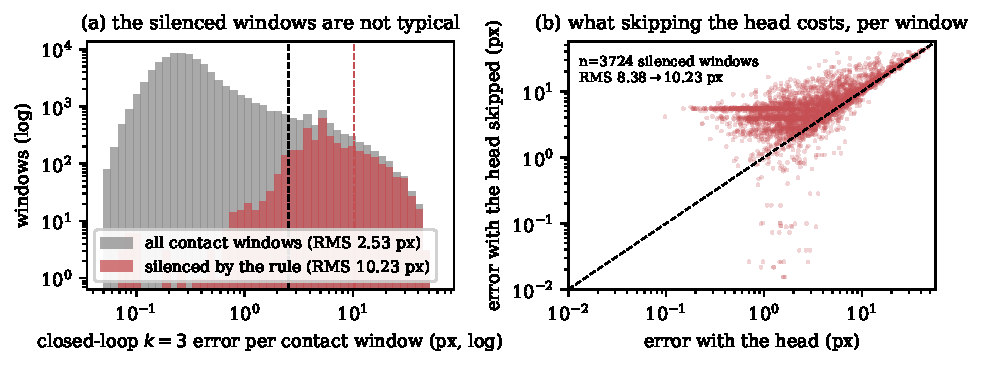
\includegraphics[width=\textwidth]{figs/fig6_silence_hist.pdf}
\caption{What the decode rule costs, window by window (nine arm--seed pairs pooled).
(a) Closed-loop error per contact window under the deployed rule; the windows it
silences (red) sit far to the right of the pool (grey), with RMS $10.23$\,px against
$2.53$\,px. (b) For the silenced windows only, the error with the head versus the error
with the head skipped; points above the diagonal are windows where skipping hurt.
Everything here is reproduced from the same code path as the S1f report, asserted
bit-identical against its stored contact RMS and false-silence rate.}
\label{fig:silence_hist}
\end{figure}

\section{Every trained arm's threshold curve}\label{app:allarms}

The preregistration for the decode rule promises the $\tau$ curves of every arm
of the study as an attachment; Figure~\ref{fig:allarms} delivers it. It sweeps
all nine trained arms under the protocol of Fig.~\ref{fig:roc} (same windows,
same rule), and the three arms of \S\ref{sec:silence}'s report reproduce
bit-identically (maximum relative difference $0.0$ at every stored grid point).
The wider sweep sharpens the reading of \S\ref{sec:silence} in two ways. First,
the trade-off is a property of the rule, not of the training recipe: all nine
arms trace the same monotone trade-off, from $\times1.01$--$1.04$ at
$\tau{=}0.5$ to $\times1.58$--$1.94$ at $\tau{=}0.95$, and their
selected thresholds span $\tau^\ast = 0.75$--$0.85$. Second, whether the landing
point buys silence is per-arm honest: six of the nine arms reach the floor on
every seed---the baseline, end-to-end-gate, supervised-gate, both-terms, F1 and
F2 arms---the reweighting arm misses on seed 42 ($0.93$ all-silenced, $0.43$\,px
against the $0.20$\,px criterion) and the closed-loop-$\times10$ arm on seed 44
($0.91$, $0.21$\,px), and the single-step $\times100$ arm, whose indicator no
longer confines its errors to the contact regime, never reaches it
($0.73$--$0.75$ all-silenced, $0.58$--$2.07$\,px). Contact damage at
$\tau^\ast$ spans $\times1.08$--$1.29$ across the nine arms, consistent with the
$1.12$--$1.21$ quoted for the report's three (\S\ref{sec:silence}); the highest
point is the supervised-gate arm's seed 42 ($\times1.29$). The per-seed curves
and verdicts are stored in \texttt{S1f\_allarms.json}.

\section{The preregistered criteria and their outcomes}\label{app:criteria}
Table~\ref{tab:criteria} lists every criterion fixed by the twelve
preregistrations, with the threshold as registered and the outcome read
from the stored report by the generating script. The gating series of
\S\ref{sec:substitute} predates those twelve and is not in the table; its
criteria are documented in its own report (\S\ref{sec:repro}). It is
included because the paper's positive claims do not exhaust what was
registered: the criteria that carry \S\ref{sec:floor} (P0a, four of four)
pass, while the preregistered threat test for the recipe (P0b-1/2/3) fails,
several closed-loop thresholds in \S\ref{sec:silence} miss as the body
reports, and one S1f robustness criterion (the indicator-training shift) was
preregistered without a stored verdict. The S1g mechanism slot, previously
unevaluated, now carries a stored report (\texttt{S1g\_report.json}).
Publishing the full ledger is the point of C6: a criterion that was
written first and then missed is evidence about the protocol, not a result
we are free to leave out.
% 由 paper/tables/build_criteria_table.py 生成；请勿手改。
\begin{table}[t]
\centering
\caption{Every preregistered criterion and its outcome (24 pass, 19 fail, 0 partial, 3 report-only, 1 not stored). Verdicts are read from the stored reports by the generating script, which aborts if any of the 19 asserted verdicts changes; the sources are \texttt{analysis\_output/}$\{$E0, P0c, S0b, S1b, S1c, S1d, S1e, S1f, S2$\}$ and \texttt{experiments/prereg\_P0b\_rollout\_recipe.json}. The headline claim of \S\ref{sec:floor} rests on P0a (4/4 pass) and the preregistered threat test P0b-1, which fails: the recipe does not close the gap. Rows marked ``not stored'' were preregistered but never given a stored verdict.}
\label{tab:criteria}
\small
\setlength{\tabcolsep}{4pt}
\begin{tabular}{@{}llp{4.6cm}l@{}}
\toprule
Slot & Criterion & Threshold (as preregistered) & Outcome \\
\midrule
P0a & monotone across the four tiers & strictly decreasing, one-step and $k{=}5$ & \cpass \\
P0a & exact tier meets absolute bar & $\le 0.10$ one-step, $\le 1.0$ $k{=}5$ & \cpass \\
P0a & beats the no-prior baseline & $k{=}5 \le 1.362$ (strong MLP) & \cpass \\
P0a & prior removes the residual burden & $\le 2\times$ the prior's one-step & \cpass \\
P0b & recipe cannot replace the prior (core threat) & strong MLP $k{=}5 \le 0.49$ in cell B & \cfail \\
P0b & pure learning rescues itself & no-prior $k{=}5 \le 1.0$ in cell B & \cfail \\
P0b & coarse prior rescues itself & coarse-prior $k{=}5 \le 2.19$ in cell B & \cfail \\
P0b & exact tier is not damaged & exact $k{=}5 \le 0.54$ in cell B & \cpass \\
P0c & label supervision main effect & $|\Delta| > 0.23$ px $\Rightarrow$ harmful & \cfail \\
P0c & prototype family main effect & $|\Delta| > 0.23$ px $\Rightarrow$ harmful & \cfail \\
P0c & interaction term & report effect and CI, no gate & \crep \\
S0b & subtraction absorbed by the exact floor & $\Delta_{one} \le +0.010$ px & \cpass \\
S0b & closed loop moves the same way & ratio $\le \times1.10$ & \cpass \\
S0b & effect-size ratio (report only) & $< 1/10 \Rightarrow$ strong absorption & \crep \\
S1 & engine cross-check & exact tier FF one-step $\le 0.01$ px & \cpass \\
S1 & ordering by computation-class distance & exact lowest, coarse highest & \cpass \\
S1 & analytic values within the float32 envelope & parabola/RK4 $\in[0.12,0.20]$, coarse $\in[0.50,0.80]$ & \cpass \\
S1 & closed loop keeps the analytic order & $k{=}5$ order $=$ one-step order & \cpass \\
S1b & trained ladder inherits the floor & exact $<$ tied pair $<$ coarse, 3/3 seeds & \cfail \\
S1b & contact frames retain headroom & mixed one-step $\le 0.80$ px & \cpass \\
S1b & trained arm reaches the silence bound & FF closed-loop $k{=}3 \le 0.50$ px & \cfail \\
S1b & exact tier not degraded & exact $\le$ parabola $\times1.10$ & \cpass \\
S1c & reweighting buys one-step silence & FF one-step $\le 0.50$ px & \cpass \\
S1c & reweighting does not damage contact & mixed one-step $\le 0.628$ px & \cpass \\
S1c & reweighting reaches the closed-loop floor & FF $k{=}3 \le 1.02$ px & \cfail \\
S1c & end-to-end gate buys silence & FF one-step $\le 0.50$ px & \cfail \\
S1d & supervised gate is fully silent & FF one-step $\le 0.10$ px (partial $\le 0.25$) & \cfail \\
S1d & supervised gate does not damage contact & mixed one-step $\le 0.628$ px & \cpass \\
S1d & supervised gate reaches the floor & FF $k{=}3 \le 0.20$ px & \cfail \\
S1d & gate accuracy & report; expected $\ge 99\%$ & \crep \\
S1d & mixed closed loop not degraded & mixed $k{=}3 \le$ baseline $\times1.10$ & \cpass \\
S1e & loss mass buys one-step silence ($\times10$ CL) & FF one-step $\le 0.10$ px & \cfail \\
S1e & loss mass does not damage contact ($\times10$ CL) & mixed one-step $\le 0.628$ px & \cpass \\
S1e & loss mass reaches the floor ($\times10$ CL) & FF $k{=}3 \le 0.20$ px & \cfail \\
S1e & both terms ($\times10$) & FF one-step $\le 0.10$, $k{=}3 \le 0.20$ & \cfail \\
S1e & single-step $\times100$ & FF one-step $\le 0.10$, $k{=}3 \le 0.20$ & \cfail \\
S1e & single-step $\times100$ does not damage contact & mixed one-step $\le 0.628$ px & \cfail \\
S1f & decode rule reaches the floor (main criterion) & val-B FF $k{=}3 \le 0.20$ px, 3/3 seeds & \cpass \\
S1f & decode rule does not damage contact & contact $k{=}3 \le$ unmasked $\times1.10$ & \cfail \\
S1f & indicator training shifts the curve & protected FF cells $\ge$ reference, 3/3 & \cns \\
S1f & ROC dominance at matched false silence & FF RMS $\le$ reference at $\pm0.5$ pp & \cpass \\
S1f & mixed closed loop not degraded & mixed $k{=}3 \le$ unmasked $\times1.10$ & \cfail \\
S1g & interference source is gradient crosstalk & head RMS $\approx 0.019$ $\Rightarrow$ crosstalk confirmed & \cpass \\
S2 & collapse reproduces across seeds & 3/3 seeds, ratio $\ge 3\times$ & \cpass \\
S2 & aliasing basin reproduces across seeds & 3/3 seeds, $\hat g \in [600,850]$ & \cpass \\
S2 & horizon causality reproduces & 3/3 seeds, $\hat g(H_1) < \hat g(H_5) < \hat g(H_{10})$ & \cpass \\
S2 & superseded truth-recovery criteria & $|\hat g/g - 1| \le 0.20$ (M-A/M-B/M-E) & \cfail \\
\bottomrule
\end{tabular}
\end{table}


\end{document}
